\documentclass[12pt,a4paper]{article}

\usepackage{mathtools, amssymb, ntheorem, amsmath, mathrsfs, hyperref, fancyhdr, geometry, framed, physics, pifont, tikz}

\geometry{a4paper, left=2cm, right=2cm, bottom=2cm, top=2cm}

\pagestyle{fancy}
\fancyhead{}
\fancyhead[L]{\leftmark}
\fancyhead[R]{\rightmark}
\fancyfoot{}
\fancyfoot[C]{\thepage}
%\renewcommand{\headrulewidth}{0pt}
\renewcommand{\footrulewidth}{0pt}

\theorembodyfont{\upshape}
\theoremseparator{.}

\newtheorem{ax}{Axiom}[section]
\newtheorem{nota}{Notation}[section]
\newtheorem{thm}{Theorem}[subsection]
\newtheorem{df}{Definition}[subsection]
\newtheorem{eg}{Example}[subsection]
\newtheorem{prop}{Proposition}[subsection]
\newtheorem{lem}{Lemma}[subsection]
\newtheorem{cor}{Corollary}[subsection]
\newtheorem{clm}{Claim}[subsection]

\newcounter{nprf}[subsection]
\setcounter{nprf}{0}
\newenvironment*{sol}{\par\indent\textbf{\textit{Solution. }}}{\hfill{$\square$}\par}
\newenvironment*{counter}{\par{\textit{Counterexample. }}}{\hfill{$\square$}\par}
\newenvironment*{ans}{\par{\textit{Answer. }}}{\hfill{$\square$}\par}
\newtheorem*{rmk}{\indent Remark}
\newenvironment*{prf}{\par\indent\textbf{\textit{Proof} (\stepcounter{nprf}\thenprf). }\par }{\par\hfill $\blacksquare$\par}
\newenvironment*{dis}{\par\indent\textbf{\textit{Disproof} (\stepcounter{nprf}\thenprf). }\par}{\par\hfill $\blacksquare$\par}
\newtheorem*{ext}{\indent Extension}

\linespread{1.25}

\hypersetup{
	colorlinks = true,
	bookmarks = true,
	bookmarksnumbered = true,
	pdfborder = 001,
	linkcolor = blue
}

\title{Emory University\\\textbf{MATH 250 - Foundations of Mathematics Learning Notes}}
\author{Jiuru Lyu}
\date{\today}

\def\Z{{\mathbb{Z}}}
\def\R{{\mathbb{R}}}
\def\Q{{\mathbb{Q}}}
\def\N{{\mathbb{N}}}
\def\Zp{{\Z^{+}}}
\def\pow{{\mathcal{P}}}
\def\part{{\mathscr{P}}}
\def\f{f^{-1}}
\def\emptyset{\varnothing}
\def\qed{\rightline{$\blacksquare$}}
\def\st{\emph{ s.t. }}
\def\fs{\emph{ f.s. }}
\def\Iff{\emph{ iff }}
\def\WTS{\mathit{WTS}}

\begin{document}
\maketitle
\tableofcontents
\newpage

\section*{Preface}
These is my personal notes for Emory University MATH 250 Foundations of Mathematics course. 

This course requires Calculus II as pre-requisite. This course focuses on Mathematical proofs and lays foundation for any other higher level math courses, such as Real Analysis, Complex Variables, Abstract Vector Space, and Abstract Algebra. The book used for this course is \textit{An Introduction to Abstract Mathematics} by Robert Bond. 

Throughout this personal note, I use different formats to differentiate different contents, including definitions, theorems, proofs, examples, extensions, and remarks. To be more specific: 
\begin{df}[Terminology]
    This is a \textbf{definition}.	
\end{df}
\begin{thm}[Theorem Name]
    This is a \textbf{theorem}.	
\end{thm}
\begin{eg}
    This is  an \textbf{example}. 
\end{eg}

\begin{ans}
    This is the \textit{answer} part of an \textbf{example}. 
\end{ans}
\begin{rmk}
	This is a \textbf{remark} of a definition, theorem, example, or proof. 
\end{rmk}

\begin{prf}
	This is a \textbf{proof} of a theorem. 
\end{prf}
\begin{ext}
	This is a \textbf{extension} of a theorem, proof, or example. 	
\end{ext}
This is a hard course, and practice will make critical thinking, mathematical thinking, and mathematical proof skills better. Even though I put efforts into making as few flaws as possible when encoding these learning notes, some errors may still exist in this note. If you find any, please contact me via email: \url{lvjiuru@hotmail.com}. 

I hope you will find my notes helpful when developing mathematical thinking skills.

\rightline{Cheers,}
\rightline{Jiuru Lyu}

\newpage
\section{Mathematical Reasoning}
\subsection{Statement}
\begin{df}[Statement]
	A \textbf{statement} is any declarative sentence that is \underline{either true or false}.
	\begin{rmk}
		A statement cannot be ambiguous, cannot be both true and false, and cannot be sometimes true or false.
	\end{rmk}
	\begin{eg}
		Examples and Non-Examples: 
		\begin{itemize}
			\item All integers are rational numbers. -- True statement
			\item $\pi$ is irrational. -- True statement
			\item $1=0.$ -- False statement
			\item $\sqrt{2}\in\Z.$ -- False statement
			\item Every student in this class is a math major. -- False statement. (To prove this false, find a student that is not a math major.)
			\item Solve the equation $2x=3.$ -- Not a statement
			\item Chocolate chip is the best ice cream flavor. -- Not a statement
			\item $x+5=3.$ -- Not a statement. (Turn it into a statement: When $x=1$, $x+5$=3; or when $x\neq-2,\ x+5\neq3.$)
		\end{itemize}
		\begin{rmk}
			$\in$ means belongs to, and $\Z$ is the notation for integers.	
		\end{rmk}
	\end{eg}
\end{df}
\begin{rmk} 
	We denote statements by letters. 
	\begin{eg}
		$P$: ``Today is a sunny day;'' $Q$: ``$3$ is a prime number.	
	\end{eg}
	If the statement's truth depends on a variable, we include the variable in the notation.
	\begin{eg}
		$R(x)$: ``$x$ is an integer;'' $P(x)$: $x+5=3$. $P(x)$ where $x\neq-2$ is false; $P(-2)$ is true.	
	\end{eg}
	\begin{eg}
		$R(f)$: ``$f$ is an increasing function.''
		\begin{itemize}
			\item If $f(x)=e^x$, then $R(f)$ is true.
			\item If $f(x)=x^2$, then $R(f)$ is false.
		\end{itemize}	
	\end{eg}
\end{rmk}
\begin{nota}[Quantifiers]
	We use the symbol $\forall$ for ``for all'' or ``for any'' and the symbol $\exists$ for ``there exists.'' $\forall$ and $\exists$ are called \textbf{quantifiers}. $\forall$ is the \textbf{universal quantifier} and $\exists$ is the \textbf{existential quantifier}.	 
	\begin{eg}
		\begin{enumerate}
			\item For any $\varepsilon>0$, there is a $\delta>0$.\[\forall\varepsilon>0,\ \exists\delta>0.\]
			\item The square of every real number is non-negative. \[\forall x\in\R,\ x^2\geq0.\]
			\item There is a real number whose square is negative. \[\exists x\in\R\st x^2<0.\]
			\item For every real number $x$, there is an integer $n$ such that $n>x$. \[\forall x\in\R,\ \exists n\in\Z\st n>x.\]
			\item For all rational numbers $x$, there exist integers $a$ and $b$ such that $x=\dfrac{a}{b}$. \[\forall x\in\Q,\ \exists a,b\in\Z\st x=\frac{a}{b}.\]
		\end{enumerate}	
	\end{eg}
	\begin{eg}
		\begin{enumerate}
			\item $\forall n\in\Z,\ \exists m\in\Z,\st m=n+5$: For every integers $n$, there exists integers $m$ such that $m=n+5$.
			\item $\forall\varepsilon>0,\ \exists\delta>0,\st\forall x,y\in\R,\text{ we have }|x-y|<\varepsilon\ \Longrightarrow\ |x^2-y^2|<\delta$: For every $\varepsilon$ greater than $0$, there exists a $\delta$ greater than $0$ such that for all real $x$ and $y$ with $|x-y|$ les than $\varepsilon$, we have $|x^2-y^2|$ is less than $\delta$. 
		\end{enumerate}
	\end{eg}
	\begin{rmk}
		$\forall\varepsilon\exists\delta$ and $\exists\delta\forall\varepsilon$ are not the same.
		
		In $\forall\varepsilon\exists\delta$, $\delta$ depends on $\varepsilon$, but $\delta$ is independent in $\exists\delta\forall\varepsilon$, meaning the same $\delta$ works for all $\varepsilon$.
		\begin{eg} 
			Compare $\forall n\in\Z,\ \exists m\in\Z\st m=n^2$ to  $\exists n\in\Z\st\forall m\in\Z,\ m=n^2.$
			\begin{ans}
				\begin{enumerate}
					\item $\forall n\in\Z,\ \exists m\in\Z\st m=n^2$: True. The square of an integer is an integer. 
					\item $\exists n\in\Z\st\forall m\in\Z,\ m=n^2.$: False: $n^2$ is just one integer and cannot be represented by all $m\in\Z$.
				\end{enumerate}
			\end{ans}
		\end{eg}
	\end{rmk}
\end{nota}
\begin{df}[Negations]
	If $P$ is a statement, the \textbf{negation} of $P$, written as $\neg P$ (read as ``not $P$'' or ``negation of $P$'') is the statement ``$P$ is false.''	
	\[\begin{cases}P\text{ is true}\\\neg P\text{ is false}\end{cases}\qquad\begin{cases}P\text{ is false}\\\neg P\text{ is true}\end{cases}\]
\end{df}
\begin{eg}
	Write the negation of $P$: ``All apples are fruits'' and check the truth value of both $P$ and $\neg P$.
	\begin{ans}
		$\neg P$: Not all apples are fruits / Some apples are not fruits / There exists an apple that is not a fruit.
		
		$P$ is true and $\neg P$ is false. 
	\end{ans}
\end{eg}
\begin{eg}
	Write the negation of $P$: ``Everyday this week was hot.''
	\begin{ans}
		$\neg P$: Somedays this week were not hot. / Not all days this week were hot. / There was a day this week that was not hot. 
	\end{ans}
\end{eg}
\begin{eg}
	$P$ all primes are odd.
	
	$\neg P$: There exists ($\exists$) a prime that is even / Some primes are not odd. (True: 2 is even.)
\end{eg}
\begin{eg}
	$Q$: $\forall x\in\R,\ x^2>x$
	
	$\neg Q$: $\exists x\in\R,\st x^2\leq x$ (True: for $x=\dfrac{1}{2},\ x^2=\frac{1}{4}<x$)	
\end{eg}
\begin{eg}
	$R$: There exists a real solution to $x^2+1=0$ / $\exists x\in\R\st x^2+1=0$
	
	$\neg R$: $\forall x\in\R,\ x^2+1\neq0$ -- (True	.)
\end{eg}
\begin{rmk}[Negating Quantifiers]
	In general: 
	\[\neg(\forall x\in S, P(x))=\exists x\in S\st\neg P(x). \]
	\[\neg(\exists x\in S, P(x))=\forall x\in S, \neg P(x). \]	
\end{rmk}
\begin{eg}
	$\exists n>0\st\forall m>0, m<n$
	
	Negation: $\forall n>0, \exists m>0\st m\geq n.$	
\end{eg}
\begin{eg}
	For all $x\in\R$, there exists a $y\in\R$,$\st xy=1$
	
	Negation: $\exists x\in\R\st\forall y\in\R,\ xy\neq1$	
\end{eg}

\subsection{Compound Statements}
\begin{df}[Conjunction and Disjunction]
	The \textbf{conjunction} of $P$ and $Q$, denoted $P\wedge Q$	, is the statement ``Both $P$ and $Q$ are true.'' The \textbf{disjunction} of $P$ and $Q$, denoted $P\vee Q$, is the statement ``$P$ is true or $Q$ is true.''
\end{df}
\begin{eg}
	Which of the following are true statements?
	\begin{enumerate}
	\item The function $x^2$ is even and it is concave up.
		
		$P$: $x^2$ is even (True), $Q$: $x^2$ is concave up (True).
		\[\therefore P\wedge Q\text{ is true.}\]
	\item Every student in this class is a math major and a human being.
		
		$P$: Every student in this class is a math major (False), $Q$: Every student in this class is a human being (True).
		\[\therefore P\wedge Q\text{ is false.}\]
	\item Every student in this class is a math major or a human being.
		\[P\vee Q\text{ is true.}\]
	\end{enumerate}
\end{eg}
\begin{eg}
	The following inequality can be written in conjunctions or disjunctions.
	\begin{enumerate}
		\item $|x|<3$: ($-3<x<3$) Conjunction: $x>-3$ AND $x<3$
		\item $|x|>3$: Disjunction: $x<-3$ OR $x>3$	
	\end{enumerate}
\end{eg}
\begin{rmk}
	$\vee$ is \textbf{inclusive or}, meaning if both $P$ and $Q$ are true, then $P\vee Q$ is also true, as opposed to \textbf{exclusive or}, meaning ``either $P$ or $Q$ but not both.''	
\end{rmk}
\begin{df}[Truth Tables]
	\textbf{Truth tables} are a handy way to organize information. 
\end{df}
\begin{eg}
	Write the truth table for the statement form: $P\vee\neg Q$.
	\begin{ans}\begin{center}\begin{tabular}{c|c|c|c}
		$P$&$Q$&$\neg Q$&$P\vee\neg Q$\\
		\hline
		T&T&F&T\\
		T&F&T&T\\
		F&T&F&F\\
		F&F&T&T
	\end{tabular}\end{center}\end{ans}
\end{eg}
\begin{df}[Logically Equivalent]
	Suppose $P$ and $Q$ are statements. We say $P$ and $Q$ are \textbf{logically equivalent}, denoted as $P\equiv Q$, if they are either both true or both false.
	
	Note: If two statements are logically equivalent, their truth values match up line by line in a truth table. We use this techniques to prove two statements mathematically (logically) equivalent. 
\end{df}
\begin{eg}
	Proving the following using truth tables.
	\begin{enumerate}
		\item $\neg(\neg P)\equiv P.$
		\begin{ans}\begin{center}\begin{tabular}{c|c|c}
		$P$&$\neg P$&$\neg(\neg P)$\\
		\hline
		T&F&T\\
		F&T&F
		\end{tabular}\end{center}\end{ans}
		\item $P\vee Q\equiv Q\vee P.$
		\begin{ans}\begin{center}\begin{tabular}{c|c|c|c}
			$P$&$Q$&$P\vee Q$&$Q\vee P$\\
			\hline
			T&T&T&T\\
			T&F&T&T\\
			F&T&T&T\\
			F&F&F&F
		\end{tabular}\end{center}\end{ans}
		\item $\neg(P\vee Q)\equiv(\neg P)\wedge(\neg Q).$
		\begin{ans}\begin{center}\begin{tabular}{c|c|c|c|c|c|c}
			$P$&$Q$&$\neg P$&$\neg Q$&$P\vee Q$&$\neg(P\vee Q)$&$(\neg P)\wedge(\neg Q)$\\
			\hline
			T&T&F&F&T&F&F\\
			T&F&F&T&T&F&F\\
			F&T&T&F&T&F&F\\
			F&F&T&T&F&T&T
		\end{tabular}\end{center}\end{ans}
		\item $P\vee(Q\vee R)\equiv(P\vee Q)\vee R.$
		\begin{ans}\begin{center}\begin{tabular}{c|c|c|c|c|c|c}
			$P$&$Q$&$R$&$Q\vee R$&$P\vee(Q\vee R)$&$P\vee Q$&$(P\vee Q)\vee R$\\
			\hline
			T&T&T&T&T&T&T\\
			T&T&F&T&T&T&T\\
			T&F&T&T&T&T&T\\
			T&F&F&F&T&T&T\\
			F&T&T&T&T&T&T\\
			F&T&F&T&T&T&T\\
			F&F&T&T&T&T&T\\
			F&F&F&F&F&F&F
		\end{tabular}\end{center}\end{ans}
	\end{enumerate}	
\end{eg}
\begin{thm}[Negating Compound Statements]
	\[\neg(P\wedge Q)=\neg P\vee\neg Q\]	
	\[\neg(P\vee Q)=\neg P\wedge\neg Q\]
\end{thm}
\begin{eg}
	It is not true that the numbers $x$ and $y$ are both even. 
	
	$P$: $x$ is even; $Q$: $y$ is even.
	
	$\neg(P\wedge Q)$: $x$ is odd ($\neg P$) OR $y$ is odd ($\neg Q$).	
\end{eg}
\begin{eg}
	It is not true that $9$ is prime or $9$ is even. 
	
	$P$: $9$ is prime; $Q$: $9$ is even.
	
	$\neg(P\vee Q)$: $9$ is not prime ($\neg P$) AND $9$ is odd ($\neg Q$)	
\end{eg}
\begin{thm}[Distributivity]
	\[P\wedge (Q\vee R)\equiv(P\wedge Q)\vee(P\wedge R)\]
	\[P\vee (Q\wedge R)\equiv(P\vee Q)\wedge(P\vee R)\]
\end{thm}
\begin{rmk}
	Truth tables can balloon in size. Indeed, if you have $P_1,\cdots,P_n$ statements involved in your statement form, your truth table will contain $2^n$ rows. 
	
	Sometimes, prove logical equivalences without using truth tables by taking advantage of the logical equivalences already proven is more approachable. 
\end{rmk}
\begin{eg}
	Prove or disprove without using ruth tables.
	\begin{enumerate}
		\item $\neg(P\wedge(\neg Q))\equiv(\neg P)\vee Q.$
			\begin{prf}
				\[\begin{aligned}
					\neg(P\wedge(\neg Q))&\equiv\neg P\vee(\neg(\neg Q))\\
					&\equiv\neg P\vee Q\qquad\text{[Negation of }\neg Q\equiv Q\text{]}
				\end{aligned}\]	
			\end{prf}

		\item $P\wedge((Q\vee R)\vee S)\equiv(P\wedge Q)\vee(P\wedge R)\vee(P\wedge S).$
			\begin{prf}
				\[\begin{aligned}
					P\wedge((Q\vee R)\vee S)&\equiv (P\wedge(Q\vee R))\vee(P\wedge S)\qquad\text{[Distributivity]}\\
					&\equiv(P\wedge Q)\vee(P\wedge R)\vee(P\wedge S)\qquad\text{[Distributivity]}
				\end{aligned}\]	
			\end{prf}
		\item $P\vee((Q\wedge R)\wedge S)\equiv(P\vee Q)\wedge(P\vee R)\wedge(P\vee S).$
			\begin{prf}
				\[\begin{aligned}
					P\vee((Q\wedge R)\wedge S)&\equiv (P\vee(Q\wedge R))\wedge(P\vee S)\qquad\text{[Distributivity]}\\
					&\equiv(P\vee Q)\wedge(P\vee R)\wedge(P\vee S)\qquad\text{[Distributivity]}
				\end{aligned}\]	
			\end{prf}
	\end{enumerate}
\end{eg}
\begin{df}[Tautology]
	A statement form that is true in all possible cases (for example, regardless of the truth values of $P$ and $Q$) is called a \textbf{tautology}.	
\end{df}
\begin{df}[Contradiction]
	A statement that is false in all possible cases (for example, regardless of the truth values for $P$ and $Q$)	is called a \textbf{contradiction}.
\end{df}
\begin{eg}
	Classify each of the following as a tautology, a contradiction, or neither.
	\begin{enumerate}
		\item $P\vee\neg P$
		\begin{center}\begin{tabular}{c|c|c}
			$P$&$\neg P$&$P\vee\neg P$\\
			\hline
			T&F&T\\
			F&T&T
		\end{tabular}$\qquad\therefore$ Tautology.\end{center}
		\item $P\wedge\neg P$
		\begin{center}\begin{tabular}{c|c|c}
			$P$&$\neg P$&$P\wedge\neg P$\\
			\hline
			T&F&F\\
			F&T&F
		\end{tabular}$\qquad\therefore$ Contradiction.\end{center}
		\item $P\vee Q$
		\begin{center}\begin{tabular}{c|c|c}
			$P$&$A$&$P\vee Q$\\
			\hline
			T&T&T\\
			T&F&T\\
			F&T&T\\
			F&F&F
		\end{tabular}$\qquad\therefore$ Neither.\end{center}
	\end{enumerate} 	
\end{eg}

\subsection{Implications}
\begin{df}[Implications or Conditional Statements]
	The symbol $\Rightarrow$ means ``implies.'' So $P\Rightarrow Q$ means ``$P$ implies $Q$'' or ``If $P$, then $Q$.''
	\begin{eg}
		\begin{itemize}
			\item If this is an apple, then it is a fruit.
			\item If a function $f$ is differentiable, then it is continuous.
		\end{itemize}	
	\end{eg}
	\begin{rmk}
		In mathematics, the truth value of an implication is \textbf{not} determined by causality. That is, the statement $P\Rightarrow Q$ means that in all circumstances in which $P$ is true, $Q$ is also true.
		\begin{center}\begin{tabular}{c|c|c}
			$P$&$Q$&$P\Rightarrow Q$\\
			\hline
			T&T&T\\
			T&F&F\\
			F&T&T\\
			F&F&T
		\end{tabular}\end{center}
		The only way for $P\Rightarrow Q$ to be false is when $P$ is true but $Q$ is false. This implies that false assumptions can lead to any conclusions. 
	\end{rmk}
\end{df}
\begin{df}{Sufficient Condition and Necessary Condition}
	If $P\Rightarrow Q$ is true, then $P$ is called a \textbf{sufficient condition} for $Q$, and $Q$ is called a \textbf{necessary condition} for $P$. There are many different ways to write $P\Rightarrow Q$in English: 
	\[P\implies Q\begin{cases}\text{If }P,\ \text{then }Q.\\Q\text{ if }P.\\Q\text{ whenever }P.\\Q,\ \text{provided that }P\\\text{Whenever }P,\text{ then also }Q.\\P\text{ is a sufficient condition for }Q.\\\text{For }Q\text{, it is sufficient that }P.\\Q\text{ is a necessary condition for }P.\\\text{For }P\text{, it is necessary that }Q.\\P\text{ only if }Q.\end{cases}\]	
\end{df}
\begin{thm}[Negation of Implications]
	Negation of an implication is a conjunction:\[\neg(P\Rightarrow Q)\equiv P\wedge\neg Q\]	
\end{thm}
\begin{eg}
	Negate the following: \[\forall\varepsilon\ \exists\delta>0,\ |x-y|<\varepsilon\implies|x^2-y^2|<\delta.\]
	\begin{ans}
		\[\exists\varepsilon\st\forall\delta>0,\ |x-y|<\varepsilon\text{ and }|x^2-y^2|\geq\delta.\]
	\end{ans}
\end{eg}
\begin{eg}
	Write in symbols and negate the statement $P$: ``For any positive $\varepsilon$ there exists a positive $M$ such that $|f(x)-b|<\varepsilon$ whenever $x>M.$''	
	\begin{ans}
		\[P:\ \forall\varepsilon>0,\ \exists M>0\st x>M\implies|f(x)-b|<\varepsilon.\]\[\neg P:\ \exists\varepsilon>0\st\forall M>0,\ x>M\text{ and }|f(x)-b|\geq\varepsilon.\]	
	\end{ans}
\end{eg}
\begin{df}[Axiom]
	An \textbf{axiom} is a statement which is regarded as being established, accepted, or self-evidently true.
\end{df}
\begin{df}[Theorem]
	A \textbf{theorem} is a statement that is true and has been verified as true.	
\end{df}
\begin{df}[Proposition]
	A \textbf{proposition} is a smaller, less important theorem.	
\end{df}
\begin{df}[Lemma]
	A \textbf{lemma} is a theorem whose main purpose is to help prove another theorem.	
\end{df}
\begin{df}[Corollary]
	A \textbf{corollary} is a result that is the immediate consequence of a theorem. 	
\end{df}
\begin{rmk}[Proving a theorem]
	Want to show ($\WTS$) $P\Rightarrow Q$: If	$P$ is false, $P\Rightarrow Q$ is automatically true, so there's nothing to show here. However, if $P$ is true, we need to show $Q$ is true (for $P\Rightarrow Q$ to be true)l.
	
	First line of a direct proof: Suppose $P$.
	
	Last line of a direct proof: Therefore $Q$.
\end{rmk}
\begin{df}[Divisibility]
	Let $a$ and $b$ be integers, with $a$ non-zero. We say $a$ \textbf{divides} $b$, written $a\mid b$, if there exists an \emph{integer} $k$ such that $b=ak$.
	
	In this case, we way that $a$ is a \textbf{factor} of $b$, and that $b$ is a \textbf{multiple} of $a$.
	
	Also note that $a\nmid b$ means that $a$ does not divide $b$. That is, $\nexists k\in\Z$, such that $b=ak$.
\end{df}
\begin{df}[Even]
	Let $n$ be integer. We say $n$ is \textbf{eve} if $2\mid n$.	
\end{df}
\begin{df}[Odd]
	Let $n$ be an integer. We say $n$ is \textbf{odd} if $2\nmid n$, $n=2k+1$, or $n=2k-1$ for some ($\fs$) $k\in\Z.$	
\end{df}
\begin{ext}
	The possible remainders if we divide an integer by $5$ is $0,\ 1,\ 2,\ 3,\ 4$, so we can suppose $n$ to be $5k,\ 5k+1,\ 5k+2,\ 5k+3,\ 5k+4$, respectively. 	
\end{ext}
\begin{ax}\label{ax1.1}
	Integers are closed under addition.	
\end{ax}
\begin{ax}\label{ax1.2}
	If $k\in\Z, (-k)\in\Z$.
\end{ax}
\begin{framed}
\noindent\texttt{Let $a,\ b$ and $c$ be integers, with $a$ non-zero. If $a\mid b$ and $a\mid c$, then $a\mid (b+c).$}
\begin{prf}
	Let $a,b,c\in\Z$ with $a\neq0$.\par Suppose $a\mid b$ and $a\mid c$. Then, by definition of divides, $\exists k,l\in\Z\st$\[b=ak\qquad\text{and}\qquad c=al.\] \par Then, $b+c=ak+al=a(k+l).$\par Since $k+l\in\Z$ (Axiom \ref{ax1.1}), by definition, $a\mid(b+c).$	
\end{prf}
\end{framed}
\begin{framed}
\noindent\texttt{Let $a$ and $b$ be integers, with $a$ non-zero. If $a\mid b$, then $a\mid(-b)$ and $(-a)\mid b$.}
\begin{prf}
	Let $a,b\in\Z$, with $a\neq0$.\par Suppose $a\mid b$. Then by definition of divides, $\exists k\in\Z\st b=ak.$\par Multiple both sides of this equation by (-1): \[-b=-ak=a(-k).\]\par Since $(-k)\in\Z,$ we get $a\mid (-b)$.$\qquad[\text{Axiom}\ref{ax1.2}]$\par Multiple $-b=a(-k)$ by $(-1)$ on both sides: \[b=(-a)(-k)\]\par Since $(-k)\in\Z,$ we see that $(-a)\mid b.$
\end{prf}	
\end{framed}
\begin{framed}
\noindent\texttt{Let $a,\ b,\ $and $c$ be integers, with $a$ and $b$ non-zero. If $(ab)\mid(ac)$, then $b\mid c.$}
\begin{prf}
	Let	$a,b,c\in\Z$ with $a\neq0$ and $b\neq0$.\par Suppose $(ab)\mid(ac)$. Then $\exists k\in\Z\st ac=(ab)k$.\par Divide both sides of the equation by $a$: \[c=bk.\]\par Since $k\in\Z$, by definition of divides, $b\mid c$.
\end{prf}
\end{framed}
\begin{framed}
\noindent\texttt{Let $n$ be an integer. If $n$ is of the form $3k+1$ for some integer $k$, then $n^2$ is again of the form $4k'+1$ for some integer $k'$.}
\begin{prf}
	Let $n\in\Z$.\par Suppose $n=3k+1\fs k\in\Z$.\par Squaring both sides: \[\begin{aligned}n^2=(3k+1)^2&=9k^2+6k+1\\&=3(3k^2+2k)+1.\end{aligned}\]\par Set $k'=3k^2+2k.$\par As $k\in\Z$, $3k^2, 2k\in\Z$, $k'=3k^2+2k\in\Z$.\par Then, $n^2$ is in the form of $3k'+1\fs k'\in\Z.$
\end{prf}
\end{framed}
\begin{framed}
\noindent\texttt{Let $n$ and $m$ be integers. If $n$ and $m$ are even, then $n+m$ is even.}
\begin{prf}
	Let $n,m\in\Z$.\par Suppose $n$ and $m$ are even. Then $\exists s,t\in\Z\st$ \[n=2s\qquad\text{and}\qquad m=2t.\]\par Then\[\begin{aligned}n+m&=2s+2t\\&=2(s+t)\end{aligned}\]\par Since $(s+t)\in\Z$, by definition, $n+m$ is even.
\end{prf}
\end{framed}
\begin{framed}
\noindent\texttt{Let $n$ and $m$ be integers. If $m$ is even, then $mn$ is even.}
\begin{prf}
	Let $n,m\in\Z.$\par Suppose $m$ is even. Then $\exists k\in\Z,\st m=2k.$\par So, $mn=(2k)n=2(kn).$\par Since $(kn)\in\Z$, by definition, $mn$ is even.	
\end{prf}
\end{framed}
\begin{df}[Parity]
	If $x$ and $y$ have the same \textbf{parity}, then $x$ and $y$ both are odd or both are even. 	
\end{df}

\begin{framed}
\noindent\texttt{If $x\in\Z$, then $x$ and $x^2$ have the same parity.}
\begin{rmk} Sometimes, it is helpful to do a case analysis!\end{rmk}
\begin{prf}
	Let $x\in\Z$\par $\boxed{\text{Case }1}$ Suppose $x$ is even.\par\hspace{5mm}Then, by definition, $x=2k\fs k\in\Z.$\par\hspace{5mm}So, $x^2=(2k)^2=4k^2=2(2k^2)$.\par\hspace{5mm}Since $(2k^2)\in\Z$, by definition, $x^2$ is even. \par $\boxed{\text{Case }2}$ Suppose $x$ is odd.\par\hspace{5mm}Then, by definition, $x=2l+1\fs l\in\Z.$\par\hspace{5mm}So, $x^2=(2l+1)^2=4l^2+4l+1=2(2l^2+2l)+1$\par\hspace{5mm}Since $(2l^2+2l)\in\Z$, by definition, $x^2$ is odd.
\end{prf}
\end{framed}

\subsection{Contrapositive and Converse}
\begin{framed}
\noindent\texttt{Let $n$ be an integer. Prove that if $3\nmid n$, then $3\mid n^2-1.$}
\begin{prf}
	Let $n\in\Z$. Suppose $3\nmid n$.\par
	$\boxed{\text{Case }1}$ Then $n=3k+1\fs k\in\Z.$\[\begin{aligned}
		n^2-1&=(3k+1)^2-1\\&=9k^2+6k+1-1\\&=9k^2+6k\\&=3(3k^2+2k)
	\end{aligned}\]\par\hspace{5mm} Since $(3k^2+2k)\in\Z$, by definition, $3\mid n^2-1.$\par 
	$\boxed{\text{Case }2}$ Then $n=3l+2\fs l\in\Z.$\[\begin{aligned}
		n^2-1&=(3l+2)^2-1\\&=9l^2+18l+4-1\\&=9l^2+18l+3\\&=3(3l^2+6l+1)
	\end{aligned}\]\par\hspace{5mm} Since $(3l^2+6l+1)\in\Z$, by definition, $3\mid n^2-1.$
\end{prf}
\end{framed}
Sometimes, we can form new implications from old ones. Let $P$ and $Q$ to be statement, and consider the implication $P\Rightarrow Q.$
\begin{df}[Converse]
	The \textbf{converse} of $P\Rightarrow Q$ is the implication $Q\Rightarrow P.$	
\end{df}
\begin{df}[Contrapositive]
	The \textbf{contrapositive} of $P\Rightarrow Q$ is the implication $\neg Q\Rightarrow\neg P.$	
\end{df}
\begin{rmk} A question that we are interested in is that ``are these equivalent to the original implication?''\end{rmk}
\begin{thm}
	\[\neg Q\Rightarrow\neg P\equiv P\Rightarrow Q.\]
	\begin{center}\begin{tabular}{c|c|c|c|c|c}
		$P$&$Q$&$P\Rightarrow Q$&$\neg P$&$\neg Q$&$\neg Q\Rightarrow\neg P$\\
		\hline
		T&T&T&F&F&T\\
		T&F&F&F&T&F\\
		F&T&T&T&F&T\\
		F&F&T&T&T&T
	\end{tabular}\end{center}
\end{thm}
Since the contrapositive of an implication is logically equivalent to the original implication, we sometimes prove the contrapositive in order to prove the original statement. 
\begin{framed}
\noindent\texttt{Prove that if the product of two integers $x$ and $y$ is even, at least one of them must be even.}
\begin{prf}
	We will prove the contrapositive: ``If $x$ and $y$ are both odd, then $xy$ is odd.''\par Let $x,y\in\Z$. Suppose $x$ and $y$ are odd.\par Then $\exists k,l\in\Z\st x=2k+1\text{ and }y=2l+1.$\par So, \[\begin{aligned}
		xy=(2k+1)(2l+1)&=4kl+2k+2l+1\\&=2(2kl+k+l)+1
	\end{aligned}\]\par Since $2kl+k+l\in\Z$, we see that $xy$ is odd.
\end{prf}	
\end{framed}
\begin{framed}
\noindent\texttt{Let $x\in\Z$. Prove that if $x^2-4x+7$ is even, then $x$ is odd. }\par
Contrapositive: If $x$ is even, then $x^2-4x+7$ is odd.
\begin{prf}
	We will prove the contrapositive.\par Let $x\in\Z$. Suppose $x$ is even. Then $x=2k\fs k\in\Z$.\par Then \[\begin{aligned}
		x^2-4x+7&=(2k)^2-4(2k)+7\\&=4k^2-8k+7\\&=2(2k^2-4k+3)+1
	\end{aligned}\]\par Since $2k^2-4k+3\in\Z$, by definition, $x^2-4x+7$ is odd. 
\end{prf}
\end{framed}
\begin{framed}
\noindent\texttt{Let $n\in\Z$. Prove that if $n^2$ is even, then $n$ is even.}\par 
Contrapositive: If $n$ is odd, then $n^2$ is odd. 
\begin{rmk}	This is a special case of Proof (2), where $x=y$ and is odd.\end{rmk}
\begin{prf}
	We will prove the contrapositive.\par Let $n\in\Z$. Suppose $n$ is odd. Then $n=2k+1\fs k\in\Z.$\par Then \[\begin{aligned}
		n^2=(2k+1)^2&=4k^2+4k+1\\&=2(2k^2+2k)+1
	\end{aligned}\]\par Since $(2k^2+2k)\in\Z$, we see $n^2$ is odd. 
\end{prf}
\end{framed}
\begin{framed}
\noindent\texttt{Prove that every even number is of the form $4k$ or $4k+2$ for some $k\in\Z.$}
\begin{prf}
	We will prove the contrapositive: If $x$ is of the form $4k+1$ or $4k+3$, then $x$ is odd. \par Suppose $x\in\Z$.\par $\boxed{\text{Case }1}$ Suppose $x=4k+1\fs k\in\Z$. \par\hspace{5mm}Then $x=4k+1=2(2k)+1$.\par\hspace{5mm}Since $2k\in\Z$, by definition, $x$ is odd. \par $\boxed{\text{Case }2}$ Suppose $x=4k+3\fs k\in\Z.$\par\hspace{5mm}Then $x=4k+3=2(2k+1)+1$\par\hspace{5mm}Since $2k+1\in\Z$, by definition, $x$ is odd. 
\end{prf}
\end{framed}
\begin{framed}
\noindent\texttt{Prove that every odd number is of the form $4k+1$ or $4k+3$ for some $k\in\Z$.}
\begin{rmk}	This implication is the converse of  as the contrapositive of the previous one. Here, the implication and the converse of it is both true.\end{rmk}
\begin{prf}
	We will prove the contrapositive: If $x$ is of the form $4k$ or $4k+2$, then $x$ is even.\par Suppose $x\in\Z.$ \par $\boxed{\text{Case }1}$ Suppose $x=4k\fs k\in\Z$. \par\hspace{5mm}Then $x=4k=2(2k)$.\par\hspace{5mm}Since $2k\in\Z$, by definition, $x$ is even. \par $\boxed{\text{Case }2}$ Suppose $x=4k+2\fs k\in\Z.$\par\hspace{5mm}Then $x=4k+=2=2(2k+1)$\par\hspace{5mm}Since $2k+1\in\Z$, by definition, $x$ is even. 
\end{prf}
\end{framed}
\begin{thm}[Prove by Contradiction]
	To prove $P$, we assume $\neg P$ and show that this implies an absurd statement (like $1=0$ or $0<0$).
\end{thm}
\begin{df}[Simplest-form]
	Let $m$ and $n$ be integers, with $n$ non-zero. We say the fraction $\dfrac{m}{n}$ is in \textbf{simplest-form} if $m$ and $n$ have no common factors.	
\end{df}
\begin{df}[Rational Numbers]
	Let $x$ be a real number. The number $x$ is said to be $\textbf{rational}$ if there exists integers $m$ and $n$, with $n$ non-zero, such that $x=\dfrac{m}{n}$.	
\end{df}
\begin{ax}
	After a finite number of cancellations, any	fraction $\dfrac{m}{n}$ can be written in simplest form. 
\end{ax}
\begin{framed}
\noindent\texttt{Prove that $\sqrt{2}$ is irrational.}
\begin{prf}
	Assume for the sake of contradiction that $\sqrt{2}$ is rational. \par Then, by definition, $\exists p,q\in\Z,$ with $q\neq0\st\sqrt{2}=\dfrac{p}{q}$. We can assume that $p$ and $q$ have no common factors. \par Note that $\sqrt{2}q=p$, squaring both sides, we see that $2q^2=p^2$.\par Since $q^2\in\Z$, by definition, $p^2$ is even. From Proof (4), if $p^2$ is even, then $p$ must be even. By definition, $\exists k\in\Z\st p=2k.$\par Plugging this back to our equation: $2q^2=(2k)^2=4k^2,$ $q^2=2k^2$.\par Since $k^2\in\Z$, we see that $q^2$ is even. Again, from Proof (4), if $q^2$ is even, then $q$ is even. \par \begin{center}$\divideontimes$ This contradicts the fact that $p,q$ had no common factors.\end{center}\par So, $\sqrt{2}$ must, in fact, be irrational. 
\end{prf}	
\end{framed}
\begin{framed}
\noindent\texttt{Let $0<\alpha<1.$ Prove that $\sqrt{\alpha}>\alpha.$}
\begin{prf}
	\textbf{We will use the Proof by Contradiction.}\par 
	Suppose $0<\alpha<1.$ Assume for the sake of contradiction that $\sqrt{\alpha}<\alpha.$\par Since $\alpha,\sqrt{\alpha}>0$ and $f(x)=x^2$ is an increasing function for positive $x$, squaring both sides, we have $\alpha\leq\alpha^2.$\par So, $\alpha^2-\alpha\geq0$. Then $\alpha(\alpha-1)\geq0.$\[\begin{cases}\alpha\geq0\\\alpha-1\geq0\end{cases}\qquad\text{or}\begin{cases}\alpha\leq0\\\alpha-1\leq0\end{cases}\]\par We have $\alpha\geq1\quad\text{or}\alpha\leq0$.\par\begin{center}$\divideontimes$ This contradicts with the fact that $0<\alpha<1.$\end{center}\par So, $\sqrt{\alpha}>\alpha.$
\end{prf}	
Another way to prove is by contrapositive.
\begin{prf}
	We will prove the contrapositive: If $\sqrt{\alpha}\leq\alpha$, then $\alpha\leq0$ or $\alpha\geq1.$\par Suppose $\alpha\in\R$ and $\sqrt{\alpha}\leq\alpha$.\par As $\sqrt{\alpha}$ exists, $\alpha\geq0.$\par Since $\alpha,\sqrt{\alpha}\geq0$ and $f(x)=x^2$ is an increasing function for $x\geq0$: $\alpha\leq\alpha^2.$ \par Then $\alpha^2-\alpha\geq0$, $\alpha(\alpha-1)\geq0$.\par Since $\alpha\geq0$, $\alpha-1$ must also be greater than $0$.\par So, we have $\begin{cases}\alpha\geq0\\\alpha-1\geq0\end{cases}$\par Hence, we have $\alpha\geq1.$
\end{prf}
\end{framed}
\begin{framed}
\noindent\texttt{Prove that there are no integer solutions to the equation $x^2=4y+2.$}
\begin{prf}	
	Assume for the sake of contradiction that $\exists x,y\in\Z\st x^2=4y+2.$\[x^2=4y+2=2(2y+1)\]\par Since $2y+1\in\Z$, $x^2$ is an even number, and thus $x$ is also an even number.\par Then, $\exists k\in\Z\st x=2k.$\[\begin{aligned}\therefore x^2=(2k)^2=4k^2&=4y+1\\2k^2&=2y+1\end{aligned}\]\par $\boxed{\text{Method }1}$\par Since $k^2\in\Z,$ $2k^2$ is even. Since $y\in\Z$, $2y+1$ is odd.\par Then the equation indicates an even number equals to an odd number.\par\begin{center}$\divideontimes$ This contradicts with the fact that even numbers cannot equal to an odd number.\end{center}\par $\boxed{\text{Method }2}$ \[\begin{aligned}2k^2&=2y+1\\2(k^2-y)&=1\\k^2-y&=\frac{1}{2}\end{aligned}\]\par\begin{center}$\divideontimes$ This contradicts with the fact that since $k,y\in\Z$, so does $k^2-y.$\end{center}\par So, our assumption is wrong. There is no integer solutions for $x^2=4y+2.$
\end{prf}
\end{framed}
\begin{df}[Prime Numbers]
	A prime number is a natural number that is only divisible by $1$ and itself.
	\begin{eg}2, 3, 5, 7, 11, 13, 17, 19, ...\end{eg}
\end{df}
\begin{framed}
\noindent\texttt{Prove there are infinitely many primes}
\begin{rmk} This is a very revealing proof by contradiction. It reveals a way to find a larger prime based on the primes that we already have. \end{rmk}
\begin{prf}
	Assume for the sake of contradiction that there are exactly $n$ primes, where $n\in\N$. Let's list them as $p_1,\ p_2,\ p_3,\cdots,p_n$, where $p_1=2,\ p_2=3,\cdots,$ $p_n$ is the largest prime.\par Consider the number $q=\underbrace{p_1p_2p_3\cdots p_n}_{\text{product}}+1$. Then notice that since $p_i\geq2\forall i$, we have $q>p_n$.\par Since $q>p_n$, $q$ cannot be prime, based on our assumption.\par So, $\exists p_k\in\{p_1,\ p_2,\ \cdots,\ p_n\}\st p_k\mid q.$ Then, by definition, $q=cp_k\fs c\in\Z.$\par So, \[c=\frac{q}{p_k}=\frac{p_1p_2p_3\cdots p_n+1}{p_k}=\frac{p_1p_2p_3\cdots p_n}{p_k}+\frac{1}{p_k}\]\par Then, \[\frac{1}{p_k}=c-\frac{p_1p_2p_3\cdots p_n}{p_k}\]\par Note that since $p_k$ is one prime among $p_1,\cdots p_n,$ $\dfrac{p_1p_2p_3\cdots p_n}{p_k}\in\Z.$\par Since $c\in\Z$, then $\dfrac{1}{p_k}\in\Z$.\begin{center}$\divideontimes$ This is a contradiction because $p_k\nmid1$ as $p_k\geq2\forall k.$\end{center}\par So, there must be infinitely many primes
\end{prf}
\end{framed}
\begin{framed}
\noindent\texttt{If $n\in\Z$, then $5n^2+3n+7$ is odd.}
\begin{prf}
	Suppose $n\in\Z$.\par $\boxed{\text{Case }1}$ If $n$ is even. Then $\exists k\in\Z\st n=2k.$ \[5n^2+3n+7=5(2k)^2+3(2k)+7=20k^2+6k+7=2(10k^2+3k+3)+1\]\par\hspace{10mm}Since $10k^2+3k+3\in\Z$, $5n^2+3n+7$ is odd.\par $\boxed{\text{Case }2}$ If $n$ is odd. Then $\exists k\in\Z\st n=2k+1$.\[5n^2+3n+7=5(2k+!)^2+3(2k+1)+7=20k^2+26k+15=2(10k^2+13k+7)+1\]\par\hspace{10mm}Since $10k^2+13k+7\in\Z$, $5n^2+3n+7$ is odd.
\end{prf}
\end{framed}
\begin{df}[Equivalence]
	The prove $P\iff Q$ (equivalence or biconditional, ``if and only if'' or ``$\Iff$'')	we must prove the forward implication $P\implies Q$ and the backward implication $Q\implies P$.
\end{df}
\begin{framed}
\noindent\texttt{Prove that for $x,y\in\R$, $(x+y)^2=x^2+y^2$ if and only if $x=0$ or $y=0$.}
\begin{prf}
	($\Rightarrow$): We will show that $(x+y)^2=x^2+y^2\implies x=0$ or $y=0$.\par\hspace{5mm}Suppose $x,y\in\Z\st(x+y)^2=x^2+y^2$. So we have \[x^2+y^2+2xy=x^2+y^2\]\par\hspace{5mm}That is, $2xy=0$ or $xy=0$. So $x=0$ or $y=0$ $\qquad\square$\par ($\Leftarrow$): We will show that $x=0$ or $y=0$ $\implies(x+y)^2=x^2+y^2$. \par\hspace{5mm}Notice that the equation retains symmetry. \par\hspace{5mm}Suppose $x,y\in\R$. Assume $x=0$ or $y=0$.\par\hspace{5mm}Without loss of generality (WLOG), we may assume that $x=0$.\par\hspace{5mm}Then, \[\begin{aligned}(x+y)^2=(0+y)^2&=y^2\\x^2+y^2=0^2+y^2&=y^2\end{aligned}\]\par\hspace{5mm}So, $(x+y)^2=x^2+y^2.$
\end{prf}
\end{framed}

\newpage
\section{Sets}

\subsection{Sets and Subsets}
\begin{df}[Set, Element]
	A \textbf{set} is a collection of objects, called \textbf{elements}. A set is typically denoted by a capital letter and a set's elements are listed in $\{\}$.
	\begin{eg}
	\begin{itemize}
		\item $A=\{1,2,3\}$
		\item $F=\{1,2,3,5,8,13,...\}$ the set of Fibonacci numbers
		\item $\N=\{1,2,3,4,5,...\}$ the \textbf{natural numbers} (Does not include $0$.)
		\item $\emptyset$ the \textbf{empty set}
		\item $M=\left\{\begin{pmatrix}1&0\\0&0\end{pmatrix},\begin{pmatrix}0&1\\0&0\end{pmatrix},\begin{pmatrix}0&0\\1&0\end{pmatrix},\begin{pmatrix}0&0\\0&1\end{pmatrix}\right\}$
		\item $\{\text{Ludacris},\text{T.I.},\text{Killer Mike},\text{Big Boi},\text{Andre 3000},\text{Latto}\}$
	\end{itemize}	
	\end{eg}
\end{df}
\begin{df}
	We write $a\in A$ ($a$ is in $A$) to indicate $a$ is an element of $A$ and $a\notin A$ ($a$ is not in $A$) to indicate $a$ is not an element of $A$.	
\end{df}
\begin{df}[Cardinality]
	The \textbf{cardinality} of a set $A$ is the number of elements in $A$ and is denoted $|A|.$
\end{df}
\begin{rmk} When listing the elements of a set, each element is listed only once (for example, $\{1,1\}$ is not a set) and the order of the elements doesn't matter ($\{1,2\}=\{2,1\}$). \end{rmk}
\begin{nota}[Set Builder Notation]
	We can use the set builder notation to describe a general property of the elements.
	\begin{eg}
		$\{2n\mid n\in\N\}$ is ``the set of elements of the form $2n$ such that $n$ is a natural number.''	
	\end{eg}
	\begin{rmk} We use $2\Z$ to represent $\{2k\mid k\in\Z\}.$ Similarly, we have $5\Z, 10\Z,...$\end{rmk}
\end{nota}
\begin{df}[Subset]
	We say a set $A$ is a \textbf{subset} of a set $B$, denoted $A\subseteq B$, if every element of $A$ is an element of $B$ (If $a\in A$, then $a\in B$). We write $A\nsubseteq B$ if $A$ is not a subset of $B$ ($\neg(A\subseteq B)=a\in A\text{ and }a\notin B.$)
	\begin{itemize}
		\item $A\subseteq B$: ``$A$ is a subset of $B$''
		\item $B\supseteq A$: ``$B$ contains $A$''
		\item $A\subsetneq B$: ``$A$ is a proper subset of $B$'' or ``$A$ is a subset of $B$, but $A\neq B$.''
	\end{itemize}
	\begin{rmk}By definition, $A\subseteq A$ (every set is a subset of itself). \end{rmk}
	\begin{rmk}$\emptyset$ is a subset of any set.\end{rmk}
\end{df}
\begin{thm}
	A set of $n$ elements has $2^n$ subsets.
	\begin{prf}
		For every element in the set, they have two options: in the subset or out the subset. Hence, there will be in total $2^n$ subsets.	
	\end{prf}
\end{thm}

\begin{df}
	Building New Sets From Old
	\begin{itemize}
		\item \textbf{Intersection}: $A\cap B=\{x\mid x\in\ A\text{ and }x\in B\}$
		\item \textbf{Union}: $A\cup B=\{x\mid x\in A\text{ or }x\in B\}$
		\item \textbf{Difference}: $A-B=A\backslash B=\{x\mid x\in A\text{ and }x\notin B\}$
	\end{itemize}
\end{df}
\begin{thm}
	\[A\cup B=B\cup A\]	
	\[A\cap B=B\cap A\]
	\[A-B\neq B-A\]
\end{thm}
\begin{df}[Universal Set]
	A \textbf{universal set} of $A$ is a set within which $A$ exists.	
\end{df}
\begin{df}[Complement]
	The \textbf{complement} of $A$ in its universal set $U$ is $\overline{A}=A^{C}=U-A.$	
\end{df}
\begin{thm}
	\[A\cup\overline{A}=U\]
	\[A\cap\overline{A}=\emptyset\]	
	Specially, if $U$ is finite, $|U|=|A|+|\overline{A}|$
\end{thm}
\begin{thm}[De Morgan's Laws]
	\[\overline{A\cup B}=\overline{A}\cap\overline{B}\]	
	\[\overline{A\cap B}=\overline{A}\cup\overline{B}\]
\end{thm}
\textbf{Set Theoretic Proofs}: Prove $a\in A$: To prove an element belongs to a set, we must prove the element satisfies the required properties of the set. 
\begin{framed}
\noindent\texttt{Prove that $14\in\{4a+7b:\ a,b\in\Z\}$}	
\begin{prf}
	Note that $14=4(0)+7(2)$\par Since $0,2\in\Z$, by definition, $14\in\{4a+7b\mid a,b\in\Z\}.$
\end{prf}
\end{framed}
\begin{thm}
	Proving $A\subseteq B$: To prove $A\subseteq B$, we must prove that if $a\in A,$ then $a\in B.$ We can do so using any technique:
	\begin{itemize}
		\item Direct proof: Suppose $a\in A$...... Therefore, $a\in B.$
		\item Contrapositive proof: Suppose $a\notin B$...... Therefore, $a\notin A.$
		\item Contradiction: Suppose $a\in A.$ Assume for the sake of contradiction that $a\in B$......$\divideontimes$
	\end{itemize}	
\end{thm}
\begin{framed}
\noindent\texttt{Prove that for all $m,n\in\Z$, we have $\{x\in\Z: mn\mid x\}\subseteq\{x\in\Z:m\mid n\}\cap\{x\in\Z:n\mid x\}.$}	
\begin{prf}
	Let $x\in\Z\st x\in\{x\in\Z: mn\mid x\}.$ Then, $mn\mid x,$ and so $x=kmn\fs k\in\Z.$\par So, $x=m(kn),$ and since $kn\in\Z$, $x\in\{x\in\Z:m\mid x\}$.\par Also, $x=n(km),$ and since $km\in\Z$, $x\in\{x\in\Z:n\mid x\}$.\par By definition of intersection, $x\in\{x\in\Z:m\mid x\}\cap\{x\in\Z:n\mid x\}$.
\end{prf}
\end{framed}
\begin{df}[Equal]
	We say two sets $A$ and $B$ are \textbf{equal}, denoted $A=B$, if they have the same elements.
	\begin{rmk}
		$A=B\iff A\subseteq B\text{ and }B\subseteq A$	
	\end{rmk}
\end{df}
\begin{framed}
\noindent\texttt{If $A$, $B$, and $C$ are sets, prove $(A\cap B)-C=(A-C)\cap(B-C)$}
\begin{prf}
	($\subseteq$): $(A\cap B)-C\subseteq(A-C)\cap(B-C)$\par\hspace{5mm}Suppose $x\in(A\cap B)-C$ ($\WTS$: $x\in(A-C)\cap(B-C)$)\par\hspace{5mm}By definition of intersection, $x\in A$ and $x\in B$\par\hspace{5mm}By definition of difference, $x\notin C.$\par\hspace{5mm}Since $x\in A$ and $x\notin C$, $x\in A-C$. Similarly, since $x\in B$ and $x\notin C$, $x\in B-C$.\par\hspace{5mm}By definition of intersection, $x\in(A-C)\cap(B-C)$ $\qquad\square$\par
	($\supseteq$): $(A-C)\cap(B-C)\subseteq(A\cap B)-C$\par\hspace{5mm}Let $x\in(A-C)\cap(B-C)$.\par\hspace{5mm}By definition of intersection, $x\in A-C$ and $x\in B-C$.\par\hspace{5mm}By definition of difference, $x\in A$, $x\notin C$ and $x\in B$, $x\notin C$.\par\hspace{5mm}Since $x\in A$ and $x\in B$, $x\in(A\cap B)$\par\hspace{5mm}Further since $x\notin C$, by definition of difference, $x\in(A\cap B)-C.$
\end{prf}
\end{framed}
\begin{framed}
\noindent\texttt{If $A$ and $B$ are sets, prove that $A\subseteq B$ if and only if $\overline{B}\subseteq\overline{A}$.}
\begin{prf}
	($\Rightarrow$): $A\subseteq B\implies\overline{B}\subseteq\overline{A}.$\par\hspace{5mm}Suppose $A\subseteq B.$ $\qquad$[WTS: $\overline{B}\subseteq\overline{A}$]\par\hspace{5mm}Suppose $x\in\overline{B}.$ $\qquad$[WTS: $x\in\overline{A}$]\par\hspace{5mm}Since $x\in\overline{B}$, then $x\notin B$. Note that since $A\subseteq B$, by definition, if $x\in A$, then $x\in B.$\par\hspace{5mm}By contrapositive, $x\notin B\implies x\notin A$\par\hspace{5mm}Since $x\notin B$, by assumption, $x\notin A$. That is $x\in\overline{A}.$$\qquad\square$\par ($\Leftarrow$): $\overline{B}\subseteq\overline{A}\implies A\subseteq B.$\par\hspace{5mm}Suppose $\overline{B}\subseteq\overline{A}$ $\qquad$[WTS: $A\subseteq B$]\par\hspace{5mm}Suppose $x\in A$ [WTS: $x\in B$]\par\hspace{5mm}Since $x\in A,$ then $x\notin\overline{A}.$ Since$\overline{B}\subseteq\overline{A}$, by contrapositive, \[x\notin\overline{A}\implies x\in\overline{B}.\]\par\hspace{5mm}Since $x\notin\overline{A},$ by assumption, $x\notin\overline{B}$. That is, $x\in B$.
\end{prf}	
\end{framed}

\subsection{Combining Sets}
\begin{framed}
\noindent\texttt{Prove that $A\subseteq B$ if and only if $A-B=\emptyset$.}
\begin{prf}
	($\Rightarrow$): WTS: $A\subseteq B\implies A-B=\emptyset$.\par\hspace{5mm}Let $A$, $B$ be sets. Suppose $A\subseteq B.$\par\hspace{5mm}Assume for the sake of contradiction that $A-B\neq\emptyset$. Then $x\in A-B$.\par\hspace{5mm}By definition of set difference, $x\in A$ and $x\notin B$.\par\begin{center}$\divideontimes$ This contradicts with the fact that $A\subseteq B$, and thus \end{center}\[A\subseteq B\implies A-B=\emptyset.\qquad\square\]\par
	($\Leftarrow$): WTS: $A-B=\emptyset\implies A\subseteq B.$\par\hspace{5mm}$\boxed{\text{Method }1}$ We will prove the contrapositive: $A\nsubseteq B\implies A-B\neq\emptyset$.\par\hspace{5mm}Suppose $A\nsubseteq B$. Then $\exists x\in A \st x\notin B$.\par\hspace{5mm}By definition of set difference, $x\in A-B,$ so $A-B\neq\emptyset$ as desired.\par\hspace{5mm}$\boxed{\text{Method }2}$ Direct proof.\par\hspace{5mm}Suppose $A-B=\emptyset$.\par\hspace{5mm}By definition of set difference, $\forall x\in A, x\in B.$\par\hspace{5mm}By definition of subsets, $A\subseteq B.$
\end{prf}	
\end{framed}
\begin{df}[Power set]
	The \textbf{power set} of $A$, denoted $\pow(A)$, is the set of all subset of $A$. Therefore, $|\pow(A)|=2^n$ when $|A|=n.$
\end{df}
\begin{thm}
	\[x\in\pow(A)\iff x\subseteq A\]	
\end{thm}
\begin{framed}
\noindent\texttt{Let $A, B$ be sets. Prove that $\pow(A)\cup\pow(B)\subseteq\pow(A\cup B)$}
\begin{prf}
	Let $A$, $B$ be sets.\par Suppose $X\in\pow(A)\cup\pow(B)$ $\big[$Notation: Capital $X$ because $X$ is a set!$\big]$\par Then, by definition of union, $X\in\pow(A)$ or $X\in\pow(B).$\par WLOG, suppose $X\in\pow(A).$ By definition of the power set, $X\subseteq A$.\par Since $A\subseteq A\cup B$, if $X\subseteq A$, then $X\subseteq A\cup B$.\par By definition of the power set, $X\in\pow(A\cup B).$\par Hence, $\pow(A)\cup\pow(B)\subseteq\pow(A\cup B).$
\end{prf}
\end{framed}
\begin{df}[Cartesian Product]
	The \textbf{Cartesian product} of two sets $A$ and $B$, denoted $A\times B$, is the set of ordered pairs (or tuples) $(a,b)$ where $a\in A$ and $b\in B$, so \[A\times B=\{(a,b)\mid a\in A, b\in B\}\]
\end{df}
\begin{rmk} In general, $A\times B\neq B\times A.$\end{rmk}
\begin{thm}
	\[|A\times B|=|A|\times|B|\]	
\end{thm}
\begin{framed}
\noindent\texttt{Let $A$, $B$, and $C$ be sets. Prove that if $B\subseteq C,$ then $A\times B\subseteq A\times C.$}
\begin{prf}
	Let $A$, $B$, and $C$ be sets. Suppose $B\subseteq C$. WTS: $A\times B\subseteq A\times C.$\par Let $x\in A\times B$. Then $x=(a,b)$ where $a\in A$ and $b\in B.$\par Since $B\subseteq C,$ if $b\in B$, then $b\in C.$\par So, $x=(a,b)\in A\times C.$\par Hence, $A\times B\subseteq A\times C.$	
\end{prf}
\end{framed}
\begin{df}[Cartesian Power]
	For a set $A$ and $n\in\N$, the \textbf{Cartesian power} $A^n$ is the set \[A^n=A\times A\times A\times\cdots\times A=\{\underbrace{(a_1,a_2,a_3,\cdots,a_n)}_{n\text{-tuple}}\mid a_1,a_2,a_3,\cdots,a_n\in A\}.\]	
\end{df}
\begin{eg}
	Most common example: the Euclidean space: $\R^n$.	
\end{eg}

\subsection{Collection of Sets}
\begin{df}[Indexed Sets]
	\[\bigcup_{i=1}^nA_i=A_1\cup A_2\cup A_3\cup\cdots\cup A_n=\{x\mid x\in A_i \fs i\}\] and \[\bigcap_{i=1}^nA_i=A_1\cap A_2\cap A_3\cap\cdots\cap A_n=\{x\mid x\in A_i\ \forall i\}\] This notation also works when we don't have specified stopping point: $\displaystyle\bigcup_{i=1}A_i=\{x\mid x\in A_i\fs i\}$ and $\displaystyle \bigcap_{i=1}A_i=\{x\mid x\in A_i\ \forall i\}$
\end{df}
\begin{eg}
	Given the indexed sets, compute the unions and intersections:
	\begin{enumerate}
		\item $A_i=[0,i)$ for $i=1,\cdots,n$
		\begin{enumerate}
			\item $\displaystyle\bigcup_{i=1}^n A_i=[0,n)$
			\begin{prf}
			Claim: $\displaystyle\bigcup_{i=1}^n A_i=[0,1).$\par($\subseteq$) Let $\displaystyle x\in\bigcup_{i=1}^n A_i.$ So, $\exists k\in\qty{1, 2,\cdots,n}\st x\in A_k$.\par\hspace{5mm}By definition of $A_k$, $x\in[0,k).$\par\hspace{5mm}That is, $0\geq x<k.$\par\hspace{5mm}Since $k\leq n,$ this inequality gives us that $0\leq x<k\leq n.$\par\hspace{5mm}So, $x\in[0,n)$ as desired. $\qquad\square$\par($\supseteq$) Let $x\in[0,n).$\par\hspace{5mm}Since $x\in[0,n),$ note that $[0,n)=A_n$.\par\hspace{5mm}So $x\in A_n$.\par\hspace{5mm}By definition of union, $x\in\displaystyle\bigcup_{i=1}^n A_i$
			\begin{rmk} To show $\displaystyle x\in\bigcup_{i=1}^n A_i$, find a specific $i$ that works. \end{rmk}	
			\end{prf}
			\item $\displaystyle\bigcap_{i=1}^n A_i=[0,1)$
			\begin{prf}
				Claim: $\displaystyle\bigcap_{i=1}^n A_i=[0,1).$\par($\subseteq$) Let $x\in\displaystyle\bigcap_{i=1}^n A_i.$\par\hspace{5mm}So, $x\in A_i\ \forall i\in\qty{1,2,\cdots,n}$.\par\hspace{5mm}Specifically, $x\in A_1=[0,1).\qquad\square$\par($\supseteq$) Let $x\in[0,1)$ $\quad$[WTS: $x\in A\ \forall i\in\qty{1,2,c\dots,n}$]\par\hspace{5mm}Let $k\in\qty{1,2,\cdots,n}.$ We will show $x\in A_k.$\par\hspace{5mm}We know that $k\geq1$ and $0\leq x<1,$ so we have $0\leq x<1\leq k.$\par\hspace{5mm}That is, $x\in[0,k).$\par\hspace{5mm}So, $x\in A_k$\par\hspace{5mm}Since $k\in\qty{1,2,\cdots,n}$ was \textbf{\textit{arbitrary}}, we have shown that $x\in A_k\ \forall k\in\qty{1,2,\cdots,n}.$\par\hspace{5mm}So, $x\in\displaystyle\bigcap_{i=1}^n A_i.$
			\end{prf}
		\end{enumerate}
		\begin{rmk} If $i\in\Z$, we have
		\begin{enumerate}
			\item $\displaystyle\bigcup_{i=1}^\infty A_i=[0,\infty)$
			\item $\displaystyle\bigcap_{i=1}^\infty A_i=[0,1)$
		\end{enumerate}\end{rmk}
		\item $A_i=[i-1,i]$ for $i=1,\cdots,n$
		\begin{enumerate}
			\item $\displaystyle\bigcup_{i=1}^n A_i=[0,n]$
			\item $\displaystyle\bigcap_{i=1}^n A_i=\begin{cases}[0,1]&\quad\text{if }n=1\\\qty{1}&\quad\text{if }n=2\\\emptyset&\quad\text{if }n>2\end{cases}$
		\end{enumerate}
		\begin{rmk}
			If $i\in\qty{1,2,\cdots}=\N,$ then we have
			\begin{enumerate}
			\item $\displaystyle\bigcup_{i=1}^\infty A_i=[0,\infty)$
			\item $\displaystyle\bigcap_{i=1}^n A_i=\emptyset$
			\end{enumerate}
		\end{rmk}
	\end{enumerate}
\end{eg}
\begin{framed}
\noindent\texttt{Prove or disprove: If $A$, $B$, and $C$ are sets, and $A\times C=B\times C,$ then $A=B.$}
\begin{prf}
	If $C=\emptyset,$ then $A\times C=\emptyset=B\times C$\par But $A$ and $B$ could be dramatically different.
\end{prf}
\end{framed}
\begin{framed}
\noindent\texttt{Prove or disprove: If $A$, $B$, and $C$ are sets, with $C\neq\emptyset$, and $A\times C=B\times C,$ then $A=B.$}
\begin{prf}
	Suppose $A$, $B$, and $C$ are sets.\par Suppose $\exists a,c\in\Z\st(a,c)=A\times C$\par By definition of Cartesian product, $a\in A$ and $c\in C.$\par Suppose $\exists b,c\in\Z\st (b,c)\in B\times C$\par Similarly, $b\in B.$\par Suppose $A\times C=B\times C.$ Then $A\times C\subseteq B\times C$ and $B\times C\subseteq A\times C$\par($\subseteq$) WTS: $A\subseteq B$.\par\hspace{5mm}If $A\times B\subseteq B\times C,$ we have $(a,c)\in B\times C$\par\hspace{5mm}Then, $a\in B.$\par\hspace{5mm}Since $a\in A,$ we know $A\subseteq B.$\par($\supseteq$) WTS: $B\subseteq A$\par\hspace{5mm}Similarly, since $B\times C\subseteq A\times C,$ we have $(b,c)\in A\times C.$\par\hspace{5mm}Then, $b\in A.$\par\hspace{5mm}Since $b\in B$, we see $B\subseteq A.$\par\hspace{5mm}By definition of set equality, $A=B.$
\end{prf}
\end{framed}

\begin{df}[Partition]\label{df2.3.2}
	Let $A$ be sets. A \textbf{partition} of $A$ is a subset of the power set of A, $\part\subseteq\pow(A)$, satisfying the following three properties:
	\begin{enumerate}
		\item If $X\in\part,$ then $X\neq\emptyset$ $\longrightarrow$ non-empty subsets of $A$
		\item $\displaystyle\bigcup_{X\in\part}X=A$
		\item If $X,Y\in\part$ and $X\neq Y,$ then $X\cap Y=\emptyset$ $\longrightarrow$ mutually disjoint.
	\end{enumerate}
\end{df}
\begin{eg}
	Let $A=\Z$ and consider the collection of subsets: \[\part=\qty{\qty{\cdots,-4,-2,0,2,4,\cdots},\qty{\cdots,-3,-1,1,3,5,\cdots}}\]	
	\begin{rmk} Divisibility partisions $\Z$: Pick $n\in\N,\ n>1.$ For every $m\in\Z$: \[m=kn+r,\] where $r$ is the remainder, and $r=\qty{0,1,2,3,\cdots,n-1}$ \end{rmk}
\end{eg}
\begin{thm}[The Pigeonhole Principle - Idea]
	You have $m$ pigeons and $n$ pigeonholes (boxes for the pigeons). If $m>n$, then there will be at least one pigeonhole with more than pigeon. If $m<n,$ then you will have at least one empty pigeonhole. 
\end{thm}
\begin{thm}[The Pigeonhole Principle]
	Let $A_1,A_2,\cdots,A_n$ be a collection of finite mutually disjoint sets. Let $\displaystyle A=\bigcup_{i=1}^n A_i.$ if $|A|=k$ and $k>n$, then $|A_i|\geq2\fs i.$	
\end{thm}
\begin{framed}
\noindent\texttt{Given any $11$ integers, there is a pair of numbers whose difference is divisible by $10$.}
\begin{prf}
	Let $\qty{a_1,a_2,\cdots,1_n}$ be $11$ integers.\par Then, $a_i=10k_i+r_i$ for $i\in\qty{1,\cdots,11}$, for $r_i=\qty{0,1,2,\cdots,9}$, and for $k_i\in\Z.$\par Then, there are $10$ possibilities for $r_i$, but there are $11$ integers.\par So, by the Pigeonhole Principle, at least $2$ integers in our list must leave the same remainder on division by $10$.\par Say: \[a_l=10k_l+r\qquad\text{and}\qquad a_m=10k_m+r\qquad\text{where}r\in\qty{0,1,2,\cdots,9}\]\par Then, \[\begin{aligned}a_l-a_m&=10k_l+r-(10k_m+r)\\&=10k_l-10k_m=10(k_l-k_m)\end{aligned}\]\par Since $k_l-k_m\in\Z,$ we say that $10\mid(a_l-a_m).$
\end{prf}	
\end{framed}
\begin{framed}
\noindent\texttt{Given $5$ points in a unit square, there are two points within $\dfrac{\sqrt{2}}{2}$ of each other.}
\begin{rmk}Think carefully about the partition that gives the result!\end{rmk}
\begin{prf}
	Split the square horizontally and vertically by picking the midpoints of each side.\begin{center}\tikzset{every picture/.style={line width=0.75pt}}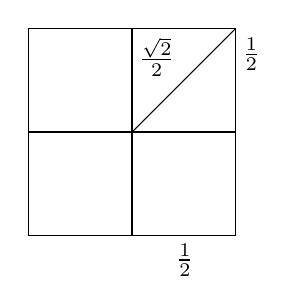
\begin{tikzpicture}[x=0.75pt,y=0.75pt,yscale=-1,xscale=1]\draw   (210.37,100.37) -- (310.37,100.37) -- (310.37,200.37) -- (210.37,200.37) -- cycle ;\draw    (210.37,150.3) -- (310.37,150.3) ;\draw    (260.37,100.3) -- (260.37,200.3) ;\draw    (310.37,100.37) -- (260.37,150.37) ;\draw (312.37,103.77) node [anchor=north west][inner sep=0.75pt]    {$\frac{1}{2}$};\draw (280.37,202.77) node [anchor=north west][inner sep=0.75pt]    {$\frac{1}{2}$};\draw (262.37,103.7) node [anchor=north west][inner sep=0.75pt]  {$\frac{\sqrt{2}}{2}$};\end{tikzpicture}\end{center}\par This divides our square into $4$ bins.\par Since there are $4$ bins and $5$ points, by the Pigeonhole Principle, at least $2$ must be in the same bin.\par Further note that in each bin, the largest distance between two points is $\dfrac{\sqrt{2}}{2}.$\par Hence, there are $2$ points with $\dfrac{\sqrt{2}}{2}$ of each other. 
\end{prf}	
\end{framed}


\newpage
\section{Functions}
\subsection{Definition and Basic Properties}
\begin{df}[Function, Domain, Codomain]
	Let $A$ and $B$ be non-empty set. A \textbf{function}, $f$, from $A$ to $B$ is a rule that assigns to each element $a\in A$ one, and only one, element of $B$, $b$.
	\begin{itemize}
		\item We call $A$ the \textbf{domain} of $f$.
		\item We call $B$ the \textbf{codomain} of $f$.
	\end{itemize}
\end{df}
\begin{nota}
	We denote a function $f$ from $A$ to $B$ as $f: A\to B,$ and the elements by $b=f(a)$ if $b$ was assigned to $a$. 	
\end{nota}
\begin{rmk}
	The codomain is part of the data that makes a function. Indeed, to specify a function, we need three pieces of information: (1) the domain, (2) the codomain, and (3) the rule between them. 
\end{rmk}
\begin{df}[Image of a Function]
	Let $f:A\to B$ be a function. The \textbf{image} of $f$, denoted $\Im{f},$ is the set of elements in the codomain which are obtained by applying the rule $f$ to an element of the domain. That is, 
	\begin{itemize}
		\item $\Im(f)=\qty{y\in B\mid\exists a\in A\st b=f(a)}$
		\item More generally, if $X\subseteq A,$ then, the \textbf{image of $X$ under }$f$, denoted $f(X)$, is given by \[f(X)=\qty{y\in B\mid\exists x\in Z\st b=f(x)}.\]
	\end{itemize}	
\end{df}
\begin{framed}
\begin{clm}Let $f:\R\to\R$ be given by $f(x)=x^2+3.$ Then $\Im(f)=[3,\infty).$\end{clm}
\begin{prf}
	($\subseteq$): Let $x\in\R.$ Then $x^2\geq0.$\par\hspace{5mm} So, $x^2+3\geq0+3.$\par\hspace{5mm} So, $\Im(f)\subseteq[3,\infty).\qquad\square$ \par 
	($\supseteq$): We will show that $(-3,\infty)\subseteq\Im(f)$\par\hspace{5mm} Let $x\in[3,\infty).\qquad$\big[WTS: $x\in\Im(f).$ That is, $\exists a\in\R\st f(a)=x.$\big]\par\hspace{5mm} Choose $a=\sqrt{x-3}.$ Since $x\geq3,\ x-3\geq0.$ So, $a\in\R.$\par\hspace{5mm} We will show that $f(a)=x$: \[f(a)=a^2+3=\qty(\sqrt{x-3})^2+3=x-3+3=x\]\par\hspace{5mm} So, $x\in\Im(f).$
\end{prf}
\end{framed}
\begin{framed}
\noindent\texttt{Let $f:\Z\to\Z$ be defined by \[f(n)=\begin{cases}n+1,\qquad n\text{ is even}\\n-3,\qquad n\text{ is odd}\end{cases}\] Compute $f(X)$ where $X=\qty{n\in\Z\mid n=4t+2\fs t\in\Z}.$}
\begin{clm}$f(X)=\qty{m\in\Z\mid m=4k+3\fs k\in\Z}=B.$\end{clm}
\begin{prf}
	($\subseteq$): Let $y\in f(X)$. Then, $\exists n\in X\st f(n)=y.$\par\hspace{5mm} By definition of $X$, $n=4t+2\fs t\in\Z.$\par\hspace{5mm} So, $f(n)=y=n+1$ since $n$ is even.\par\hspace{5mm} That is, $f(n)=y=4t+2+1=4t+3.$\par\hspace{5mm} So, $y\in B$\par 
	($\supseteq$): Let $m\in B.$ Then, $m=4k+3\fs k\in\Z.\qquad$\big[WTS: $m\in f(X)$\big]\par\hspace{5mm} Note that since $k\in\Z,$ $4k+2\in X.$ Choose $n=4k+2.$\par\hspace{5mm} Then, $n\in X.$ Further, $f(n)=n+1=4k+2+1=4k+3=m.$\par\hspace{5mm} So, $m\in f(X).$
\end{prf}
\end{framed}
\begin{thm}[Intermediate Value Theorem]\label{thm3.1.1}
	Let $f$ be a function whose domain and codomain are subsets of $R.$ Let $a<b$ and suppose $f$ is continuous on $[a,b].$ If $y$ is any number in-between $f(a)$ and $f(b),$ then there exists a number $c$ in $[a,b]$ such that $f(c)=y.$
\end{thm}
\begin{framed}
\noindent\texttt{Let $f:\R\to\R$ be given by $f(x)=x^3+x+1.$ Let $X=[-2,2].$ Then, $f(X)=[-9,11].$}
\begin{prf}
	($\subseteq$): First observe that $f'(x)=3x^2+1>0.$\par\hspace{5mm} Since $f'>0,$ $f$ is increasing. So, $f$ is in particular increasing on $[-2,2].$\par\hspace{5mm} Note that $f(-2)=(-2)^3+(-2)+1=-8-2+1=-9.$\par\hspace{5mm} Also, $f(2)=2^3+2+1=11.$\par\hspace{5mm} Since $f$ is increasing, $\forall x\in[-2,2], -9\leq f(x)\leq11.$\par\hspace{5mm} So, $f(X)\subseteq[-9,11].\qquad\square$ \par
	($\supseteq$):Let $m\in[-9,11].$\par\hspace{5mm} Since $f$ is continuous on $[-2,2]$ and $f(-2)=9$ and $f(2)=11.$\par\hspace{5mm} By the intermediate value theorem (Theorem \ref{thm3.1.1}), $\exists c\in[-2,2]\st f(c)=m.$\par\hspace{5mm} That is, $m\in f(X).$
\end{prf}	
\end{framed}
\begin{framed}
\noindent\texttt{Let $f:\R\to\R$ be given by $f(x)=x^3-4x+1.$ Let $X=[-2,2].$ Find $f(X).$}
\begin{prf}
	\begin{enumerate}
		\item[\ding{172}] Find $f'(x)=3x^2-4.$ So, $f$ is not always increasing or decreasing.
		\item[\ding{173}] Find critical points: $f'(x)=0,\ 3x^2-4=0,\ 3x^2=4,\ x^2=\dfrac{4}{3},\ x=\pm\dfrac{2}{\sqrt{2}}.$
		\item[\ding{174}] Plug in critical points into $f''(x):\ f''(x)=6x.$
		\begin{itemize}
			\item $f''\qty(\dfrac{2}{\sqrt{3}})=6\qty(\dfrac{2}{\sqrt{3}})>0\longrightarrow$ minimum
			\item $f''\qty(-\dfrac{2}{\sqrt{3}})=6\qty(-\dfrac{2}{\sqrt{3}})<0\longrightarrow$ maximum
		\end{itemize}
	\end{enumerate}
	\begin{itemize}
		\item Largest output is at $-\dfrac{2}{\sqrt{3}}$ or at $2$.\par $f(2)=2^3-4(2)+2=1$\par $f\qty(-\dfrac{2}{\sqrt{3}})=\qty(-\dfrac{2}{\sqrt{3}})^3-4\qty(-\dfrac{2}{\sqrt{3}})+1=\dfrac{8}{\sqrt{3}}\qty(\dfrac{2}{3})+1>1$
		\item Smallest output is at $-2$ or $\dfrac{2}{\sqrt{3}}.$\par $f(-2)=(-2)^3-4(-2)+2=1$\par $f\qty(\dfrac{2}{\sqrt{3}})=\qty(\dfrac{2}{\sqrt{3}})^3-4\qty(\dfrac{2}{\sqrt{3}})+1=\dfrac{8}{\sqrt{3}}\qty(-\dfrac{2}{3})+1<1$
	\end{itemize}
	Therefore, $f([-2,2])=\qty[1-\dfrac{2}{3}\qty(\dfrac{8}{\sqrt{3}}), 1+\dfrac{2}{3}\qty(\dfrac{8}{\sqrt{3}})]$
\end{prf}	
\end{framed}
\begin{thm}
	Let $f:A\to B$ be a function, and let $X$ and $Y$ be subsets of $A$. Then: 
	\begin{enumerate}
		\item\label{thm3.1.2a} $f(X\cup Y)=f(X)\cup f(Y)$
		\item\label{thm3.1.2b} $f(X\cap Y)\subseteq f(X)\cap f(Y)$
	\end{enumerate}	
\end{thm}
\begin{framed}
\noindent\texttt{We will prove Theorem 3.2.1(\ref{thm3.1.2a}) in this section. Theorem 3.2.1(\ref{thm3.1.2b}) is left as an exercise. }
\begin{prf}
	($\subseteq$): Let $b\in f(X\cup Y).$\par\hspace{5mm} Then, $\exists a\in X\cup Y\st f(a)=b.$\par\hspace{5mm} Since $a\in X$ and $f(a)=b,$ by definition of image, $b\in f(X).$\par\hspace{5mm} Then, $b\in f(X)\cup f(Y).\qquad\square$\par 
	($\supseteq$): Suppose $b\in f(X)\cup f(Y).$\par\hspace{5mm} Then, $b\in f(X)$ or $b\in f(Y).$\par\hspace{5mm} WLOG, suppose $b\in f(X).$\par\hspace{5mm} Then, $\exists a\in X\st f(a)=b.$\par\hspace{5mm} Since $a\in X,$ $a\in X\cup Y.$ So, $b=f(a)\in f(X\cup Y).$
\end{prf}
\end{framed}
\begin{rmk}
	Give a function $f:A\to B$ and subsets $X,Y\subseteq A,$ it is not true, in general, that $f(X\cap Y)=f(X)\cap f(Y).$ 
\end{rmk}
\begin{df}[Inverse Image, or Pre-Image]
	Let $f:A\to B$ be a function, and let $W\subseteq B.$ The \textbf{inverse image} of $W$ with respect to $f$ denoted $f^{-1}(W),$ is the set of elements in the domain which are sent, by applying the rule $f$, to an element of $W$ in $B$. That is, \[f^{-1}(W)=\qty{a\in A\mid f(a)\in W}.\]
	\begin{rmk}
	\begin{enumerate}
		\item $f(X)\subseteq B$ but $f^{-1}(W)\subseteq A.$
		\item To show $y\in f(X),$ \textbf{find} an $a\in X\st f(a)=y.$
		\item To show $y\in f^{-1}(W),$ \textbf{show} $f(y)\in W.$
		\item $y\in f^{-1}(W)\iff f(y)\in W.$
		\item If $f(X)=f(Y)$, we cannot determine if $X=Y.$
		\item $f^{-1}(B)=A,$ but $f(A)\neq B.$
		\item If $f^{-1}(X)=f^{-1}(Y),$ we cannot determine if $X=Y.$
	\end{enumerate}
	\end{rmk}
\end{df}
\begin{framed}
\noindent\texttt{Suppose $f:\R\to\R$ is defined by $f(x)=3x+1.$}
\begin{clm}$\f(W_2)=(1,\infty),$ where $W_2=(4,\infty)$\end{clm}
\begin{prf}
	($\subseteq$): Let $x\in f^{-1}(W_2).$\par\hspace{5mm} Then, $f(x)\in W_2=(4,\infty)$\par\hspace{5mm} So, $f(x)=3x+1>4.$ So, $x>1.$\par\hspace{5mm} That is, $x\in(1,\infty).\qquad\square$\par 
	($\supseteq$): Let $x\in(1,\infty).\qquad$\big[WTS: $x\in f^{-1}(W_2).$\big]\par\hspace{5mm} Since $x>1,$ so $3x>3$ and $3x+1>4.$\par\hspace{5mm} That is, $f(x)>4.$\par\hspace{5mm} So, $f(x)\in W_2,$ or $x\in f^{-1}(W_2).$
\end{prf}
\begin{clm}$f^{-1}(W_4)=X,$ where $W_4=\Z$ and $X=\qty{\dfrac{k-1}{3}\mid k\in\Z}.$\end{clm}
\begin{prf}
	($\subseteq$): Let $x\in f^{-1}(W_4).$\par\hspace{5mm} So, $f(x)\in W_4.$ That is, $f(x)\in\Z.$\par\hspace{5mm} Hence, $3x+1=k\fs k\in\Z.$\par\hspace{5mm} Therefore, $x=\dfrac{k-1}{3}.$ So, $x\in X.\qquad\square$\par 
	($\supseteq$): Let $x\in X.$\par\hspace{5mm} Then, $x=\dfrac{k-1}{3}\fs k\in\Z.\qquad$\big[WTS: $x\in f^{-1}(W_4)$. WTS: $f(x)\in W_4$\big]\par\hspace{5mm} $f(x)=f\qty(\dfrac{k-1}{3})=3\qty(\dfrac{k-1}{3})+1=k-1+1=k.$\par\hspace{5mm} Since $k\in\Z,$ $f(x)\in\Z=W_4.$\par\hspace{5mm} So, $x\in f^{-1}(W_4).$
\end{prf}
\end{framed}
\begin{thm}
	Let $f:A\to B$ be a function, and let $W$ and $Z$ be subsets of $B$. Then: 
	\begin{enumerate}
		\item\label{thm3.1.3(1)} $\f(W\cup Z)=\f(W)\cup \f(Z)$
		\item\label{thm3.1.3(2)} $\f(W\cap Z)=\f(W)\cap \f(Z)$
	\end{enumerate}	
\end{thm}
\begin{framed}
\noindent\texttt{We will prove Theorem 3.1.3(\ref{thm3.1.3(1)}) in this section. Theorem 3.1.3(\ref{thm3.1.3(2)}) is left as an exercise.}
\begin{prf}
	($\subseteq$): Let $y\in\f(W\cup Z).$ Then, $f(y)\in W\cup Z.$\par\hspace{5mm} By definition of union, $f(y)\in W$ or $f(y)\in Z.$\par\hspace{5mm} WLOG, suppose $f(y)\in W.$ Then, $y\in\f(W).$\par\hspace{5mm} But $\f(W)\subseteq\f(W)\cup\f(Z).$\par\hspace{5mm} So, $y\in\f(W)\cup\f(Z).\qquad\square$\par 
	($\supseteq$): Let $y\in\f(W)\cup\f(Z).$ By definition of union, $y\in\f(W)$ or $y\in\f(Z).$\par\hspace{5mm} WLOG, suppose $y\in\f(W).$ Then, $f(y)\in W.$\par\hspace{5mm} But, $W\subseteq W\cup Z.$ So, $f(y)\in W\cup Z.$\par\hspace{5mm} So, $y\in\f(W\cup Z).$
\end{prf}
\end{framed}
\begin{df}[Epsilon-Delta Definition of Continuity]\label{df3.1.4}
	Let $A$ and $B$ be open intervals of $\R$, and let $f:A\to B$ be a function. Let $a\in A.$ We say $f$ is \textbf{continuous at} $a$ if the following statement is true: \[\forall\varepsilon>0,\ \exists\delta>0\st|x-a|<\delta\implies|f(x)-f(a)|<\varepsilon.\]
	\begin{rmk} The following statement can be also rephrased as ``If $x\in(a-\delta,a+\delta),$ then $f(x)\in(f(a)-\varepsilon,f(a)+\varepsilon).$''\end{rmk}
	\begin{enumerate}
		\item $|x-a|<\delta$ means the inputs are at most $\delta$ away from $a$.
		\item $|f(x)-f(a)|<\varepsilon$ means the outputs are at most $\varepsilon$ away from $f(a)$.	
	\end{enumerate}
	\begin{rmk}
		The idea of writing a proof: given $\varepsilon>0,$ FIND $\delta>0$ that works.	
	\end{rmk}
\end{df}
\begin{framed}
\noindent\texttt{Use the formal definition of continuity (Definition \ref{df3.1.4}) to show that $f(x)=2x+1$ is continuous at $x=3$. }
\begin{prf}
	Let $\varepsilon>0$ be given. Choose $\delta=\dfrac{\varepsilon}{2}>0.$\par Suppose $x\in\R\st |x-3|<\delta.$\par Then, \[\begin{aligned}|f(x)-f(3)|&=|2x+1-7|\\&=|2x-6|\\&=|2(x-3)|\\&=2|x-3|<2\cdot\delta=2\cdot\dfrac{\varepsilon}{2}=\varepsilon.\end{aligned}\]\par Since $\varepsilon>0$ was arbitrary, we've shown that \[\forall\varepsilon>0,\ \exists\delta>0\st|x-3|<\delta\implies|f(x)-f(3)|<\varepsilon.\]
\end{prf}
\end{framed}
\begin{framed}
\noindent\texttt{Use the formal definition of continuity (Definition \ref{df3.1.4}) to show that $f(x)=3+5x$ is continuous at $x=4$. }
\begin{prf}
	Let $\varepsilon>0$ be given. Choose $\delta=\dfrac{\varepsilon}{5}>0.$\par Suppose $x\in\R\st|x-4|<\delta.$\par Then, \[\begin{aligned}|f(x)-f(4)|&=|3+5x-23|\\&=|5x-20|\\&=|5(x-4)|\\&=5|x-4|<5\cdot\delta=5\cdot\dfrac{\varepsilon}{5}=\varepsilon\end{aligned}\]\par Since $\varepsilon>0$ was arbitrary, we've shown that \[\forall\varepsilon>0,\ \exists\delta>0\st|x-4|<\delta\implies|f(x)-f(4)|<\varepsilon.\]
\end{prf}
\begin{rmk} In this example, $\delta$ ONLY depends on $\varepsilon$! So, the same $\delta$ will work when showing $f(x)$ is continuous at $x=1.$\end{rmk}
\end{framed}
\begin{framed}
\noindent\texttt{Use the formal definition of continuity (Definition \ref{df3.1.4}) to show that $f(x)=x^2$ is continuous at $x=0$.}
\begin{prf}
	Let $\varepsilon>0$ be given. Choose $\delta=\sqrt{\varepsilon}.$\par Note that since $\varepsilon>0,$ $\delta>0.$\par Suppose $x\in\R\st|x-0|<\delta.$ That is, $|x|<\delta.$\par Then, \[\begin{aligned}
		|f(x)-f(0)|=|x^2-0|=|x^2|&=|x|\cdot|x|\\&<\delta\cdot\delta=\qty(\sqrt{\varepsilon})\cdot\qty(\sqrt{\varepsilon})=\varepsilon.\end{aligned}\]\par Since $\varepsilon>0$ was arbitrary, we've shown that \[\forall\varepsilon>0,\ \exists\delta=\sqrt{\varepsilon}>0\st|x-0|<\delta\implies|f(x)-f(0)|<\varepsilon.\]	
\end{prf}

\end{framed}




\newpage
\section{Binary Operations and Relations}
\subsection{Binary Operations}
\subsection{Equivalence Relations}
\begin{df}[Relation]
	A \textbf{relation} $R$	 on a set $A$ is a subset of $A\times A=\qty{\qty(a,b)\mid a,b\in A.}$ 
\begin{nota}
	If two elements $a,b\in A$ are related, we write $(a,b)\in R$ or $aRb.$ If $a$ and $b$ are not related, we write $(a,b)\notin A$ or $a\not Rb.$
\end{nota}
\end{df}
\begin{ext} More generally, if $A$ and $B$ are sets, then a relation $R$ from $A$ to $B$ is a subset of $A\times B.$\end{ext}

\begin{eg}
Describe the following relations by listing the elements of the relation
\begin{enumerate}
	\item Let $A=\qty{1,2,3,4,5}$ and $R_<$ is the relation ``strictly less than.''
	\begin{ans}
		$aRb$ if $a<b.$ \[R_<=\qty{(1,2),(1,3),(1,4),(1,5),(2,3),(2,4),(2,5),(3,4),(3,5),(4,5)}.\]	
	\end{ans}
	\item Let $A=\qty{1,2,3,4,5}$ and $R_\mid$ is the relation ``divides.''
	\begin{ans}
		\[R_\mid=\qty{(1,1),(1,2),(1,3),(1,4),(1,5),(2,2),(2,4),(3,3),(4,4),(5,5)}.\]	
	\end{ans}
	\item Let $A=\R$ and $R=\qty{(x,y)\in\R\times\R\mid x=y}$.
	\begin{ans}
		This relation describes the line of $y=x$ in a Cartesian plane.	
	\end{ans}
	\begin{rmk}
		Any subset of $A\times A$ is a relation. A relation does not have to have a actual meaning such as ``strictly less than'' or ``divides.''	
	\end{rmk}
\end{enumerate}	
\end{eg}
\begin{df}[Reflexive, Symmetric, Antisymmetric, Transitive]
	A relation $R$ on a set $A$ is \begin{itemize}
 	\item \textbf{\underline{Reflexive}} if $(a,a)\in R\quad\forall a\in A.$
 	\begin{prf}
 		Suppose $a\in A.$ We'll show that $(a,a)\in R.$
 	\end{prf}
 	\begin{dis}
 		$\exists a\in A\st(a,a)\notin R.$
 	\end{dis}
 	\item \textbf{\underline{Symmetric}} if $\forall a,b\in A,$ if $(a,b)\in R$,then $(b,a)\in R.$
 	\begin{prf}
 		Suppose $a,b\in A.$ Suppose $(a,b)\in R.$\par We'll show that $(b,a)\in R.$
 	\end{prf}
 	\begin{dis}
 		$\exists a,b\in A\st(a,b)\in R$ and $(b,a)\notin R.$
 	\end{dis}
 	\item \textbf{\underline{Antisymmetric}} if $\forall a,b\in A,$ if $(a,b)\in R$ and $(b,a)\in R,$ then $a=b.$
 	\begin{prf}
 		Suppose $a,b\in A.$ Suppose $(a,b)$ and $(b,a)\in R.$\par We'll show that $a=b.$
 	\end{prf}
 	\begin{dis}
 		$\exists a,b\in A\st (a,b)$ and $(b,a)\in R$ and $a\neq b.$
 	\end{dis}
 	\item \textbf{\underline{Transitive}} if $\forall a,b,c\in A,$ if $(a,b)\in R$ and $(b,c)\in R,$ then $(a,c)\in R.$
 	\begin{prf}
 		Suppose $a,b,c\in A.$ Suppose $(a,b)$ and $(b,c)\in R$\par  We'll show that $(a,c)\in R.$
 	\end{prf}
\end{itemize}\end{df}
\begin{eg}
Show if the following relations are reflexive, symmetric, antisymmetric, or transitive.
\begin{enumerate}
	\item Suppose $A\subseteq\Z$ or $\N$. Consider $R_<$. 
	\begin{itemize}
		\item \textbf{\underline{Reflexive}}: False.
		\begin{counter}
			$(1,1)\notin R_<.$	
		\end{counter}
		\item \textbf{\underline{Symmetric}}: False.
		\begin{counter}
			$(1,2)\in R_<,$ but $(2,1)\notin R_<.$
		\end{counter}
		\item \textbf{\underline{Antisymmetric}}: True.
		\begin{prf} Impossible for $(a,b)$ and $(b,a)\in R.$ So the assumption part of the implication is wrong, which means the implication overall is true. \end{prf}
		\item \textbf{\underline{Transitive}}: True
		\begin{prf}
			Suppose $a,b,c\in A\st a<b,\ b<a$\par Then, $a<c.$ That is, $(a,c)\in R.$
		\end{prf}
	\end{itemize}
	\item Suppose $A\subseteq\Z$ or $\N$. Consider $R_|$.
	\begin{itemize}
		\item \textbf{\underline{Reflexive}}: True
		\begin{prf}
			Recall that $a\mid b$ if $b=ak\fs k\in\Z.$\par So, when $k=1,$ $b=a.$ That is, $a\mid a\forall a\in Z.$\par That is, $(a,a)\in R.$
		\end{prf}
		\item \textbf{\underline{Symmetric}}: False.
		\begin{counter}
			$(1,2)\in R_|,$ but $(2,1)\notin R_|.$	
		\end{counter}
		\item \textbf{\underline{Antisymmetric}}: True if $A=\N$; False if $A=\Z.$
		\begin{prf}
			Suppose $a,b\in A\st a\mid b$ and $b\mid a$.\par Then, $b=ak$ and $a=bl\fs k,l\in\Z.$\par So, $a=(ak)l=akl.$ \[\begin{aligned}a-akl&=0\\a(1-kl)&=0\\a=0\qquad\text{ or }&\qquad kl=1\\&k=l=1\quad\text{ or }\quad k=l=-1.\end{aligned}\] That is, $a=0$ or $a=b$ or $a=-b.$ So the relation is antisymmetric if $A=\N$ because then only the option $a=b$ makes sense. If $A=\Z,$ all three options are possible. 
		\end{prf}
		\item \textbf{\underline{Transitive}}: True.
		\begin{prf}
			$a\mid b\implies b=ak\qquad b\mid c\implies c=bl$\par $\implies c=(ak)l=a(kl)\implies a\mid c.$
		\end{prf}
	\end{itemize}
	\item Consider the relation $R=\qty{(x,y)\in R^2\mid x^2+y^2=1}.$
	\begin{itemize}
		\item \textbf{\underline{Reflexive}}: False.
		\begin{counter}
			$(0,0)\notin R$ because $0^2+0^2\neq1.$
		\end{counter}
		\item \textbf{\underline{Symmetric}}: True
		\begin{prf}
			Let $x,y\in\R\st xRy.$ Then, $x^2+y^2=1.$\par Then, $y^2+x^2=1$. That is, $yRx.$
		\end{prf}
		\item \textbf{\underline{Antisymmetric}}: False.
		\begin{counter}
			Consider $\qty(\dfrac{1}{2},\dfrac{\sqrt{3}}{2})$ and $\qty(\dfrac{\sqrt{3}}{2}, \dfrac{1}{2})\in R,$ but $\dfrac{\sqrt{3}}{2}\neq\dfrac{1}{2}$\par Or, consider $\qty(0,1)$ and $(1,0)\in R,$ but $0\neq1.$
		\end{counter}
		\item \textbf{\underline{Transitive}}: False.
		\begin{counter}
			$(0,1)\in R$ and $(1,0)\in R,$ but $(0,0)\notin R.$
		\end{counter}
	\end{itemize}
	\item Consider the relation $R_\leq=\qty{(x,y)\in\R^2\mid x\leq y}$.
	\begin{itemize}
		\item \textbf{\underline{Reflexive}}: True. 
		\item \textbf{\underline{Symmetric}}: False.
		\begin{counter}
			$(1,2)\in R,$ but $(2,1)\notin R.$	
		\end{counter}
		\item \textbf{\underline{Antisymmetric}}: True.
		\begin{prf}
			If $a\leq b$ and $b\leq a,$ then $a=b.$
		\end{prf}
		\item \textbf{\underline{Transitive}}: True.
		\begin{prf}
			If $a\leq b$ and $b\leq c,$ then $a\leq c.$	
		\end{prf}
	\end{itemize}
	\item Let $S$ be the set of all finite subsets of $\Z.$ Consider the relation $R$ on $S$ by $ARB$ if $\qty|A|=\qty|B|.$
	\begin{itemize}
		\item \textbf{\underline{Reflexive}}: True.
		\begin{prf} $\qty|A|=\qty|A|.$\end{prf}
		\item \textbf{\underline{Symmetric}}: True.
		\begin{prf} If $\qty|A|=\qty|B|,$ then $\qty|B|=\qty|A|.$\end{prf}.
		\item \textbf{\underline{Antisymmetric}}: False.
		\begin{counter}
			If $A=\qty{1,2}$ and $B=\qty{2,3},$ then $\qty|A|=\qty|B|,$ but $A\neq B.$	
		\end{counter}
		\item \textbf{\underline{Transitive}}: True.
		\begin{prf}
			If $\qty|A|=\qty|B|$ and $\qty|B|=\qty|C|,$ then $\qty|A|=\qty|C|.$ 	
		\end{prf}
	\end{itemize}
\end{enumerate}
\end{eg}
\begin{df}[Equivalence Relation]
	A relation $R$ on a set $A$ is an \textbf{equivalence relation} on $A$ if it is \underline{reflexive, symmetric, and transitive}. 
\begin{nota}
	When $R$ is an equivalence relation, it is common to write $a\sim b$ (read as ``$a$ is equivalent to $b$'') instead of $aRb.$
\end{nota}
\begin{rmk} Equivalence relations are a way to generalize the idea of ``equality.'' \end{rmk}
\end{df}
\begin{framed}
\noindent\texttt{Prove that $R_=$ on the set $\R$ is an equivalence relation.}
\begin{prf}
	\begin{itemize}
		\item \textbf{\underline{Reflexive}}: $a=a\quad\forall a\in\R$
		\item \textbf{\underline{Symmetric}}: $a=b\implies b=a\quad\forall a,b\in\R.$
		\item \textbf{\underline{Transitive}}: $a=b,\ b=c\implies a=c\quad\forall a,b,c\in\R.$
	\end{itemize}
\end{prf}
\end{framed}
\begin{rmk}	We can use graphs and arrows to represent a relation. 
	\begin{itemize}
		\item \textbf{\underline{Reflexive}}: Every vertex needs a self loop.
		\item \textbf{\underline{Symmetric}}: Every edge that is not a loop should look like $\Longleftrightarrow$
		\item \textbf{\underline{Transitive}}: We should have something like vector addition for every three vertexes. 
	\end{itemize}
	\begin{eg}
		The relation $R=\qty{(1,1),(2,2),(2,4),(3,2),(3,3),(4,3),(4,4)}$ on the set $A=\qty{1,2,3,4)}$ as the follwoing graph: 
		\begin{center}
		\tikzset{every picture/.style={line width=0.75pt}}
		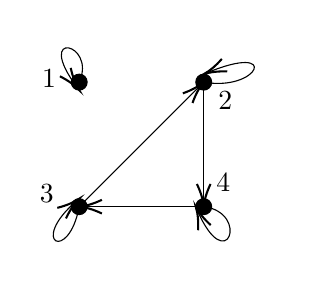
\begin{tikzpicture}[x=0.75pt,y=0.75pt,yscale=-1,xscale=1]
		\draw  [fill={rgb, 255:red, 0; green, 0; blue, 0 }  ,fill opacity=1 ] (136.36,20.46) .. controls (136.36,18.35) and (138.07,16.63) .. (140.18,16.63) .. controls (142.29,16.63) and (144,18.35) .. (144,20.46) .. controls (144,22.57) and (142.29,24.28) .. (140.18,24.28) .. controls (138.07,24.28) and (136.36,22.57) .. (136.36,20.46) -- cycle ;
		\draw  [fill={rgb, 255:red, 0; green, 0; blue, 0 }  ,fill opacity=1 ] (136.36,80.46) .. controls (136.36,78.35) and (138.07,76.63) .. (140.18,76.63) .. controls (142.29,76.63) and (144,78.35) .. (144,80.46) .. controls (144,82.57) and (142.29,84.28) .. (140.18,84.28) .. controls (138.07,84.28) and (136.36,82.57) .. (136.36,80.46) -- cycle ;
		\draw  [fill={rgb, 255:red, 0; green, 0; blue, 0 }  ,fill opacity=1 ] (196.36,20.46) .. controls (196.36,18.35) and (198.07,16.63) .. (200.18,16.63) .. controls (202.29,16.63) and (204,18.35) .. (204,20.46) .. controls (204,22.57) and (202.29,24.28) .. (200.18,24.28) .. controls (198.07,24.28) and (196.36,22.57) .. (196.36,20.46) -- cycle ;
		\draw  [fill={rgb, 255:red, 0; green, 0; blue, 0 }  ,fill opacity=1 ] (196.36,80.46) .. controls (196.36,78.35) and (198.07,76.63) .. (200.18,76.63) .. controls (202.29,76.63) and (204,78.35) .. (204,80.46) .. controls (204,82.57) and (202.29,84.28) .. (200.18,84.28) .. controls (198.07,84.28) and (196.36,82.57) .. (196.36,80.46) -- cycle ;
		\draw    (140.18,20.46) .. controls (148.87,1.57) and (117.96,-5.51) .. (139.17,22.95) ;
		\draw [shift={(140.18,24.28)}, rotate = 232.32] [color={rgb, 255:red, 0; green, 0; blue, 0 }  ][line width=0.75]    (10.93,-3.29) .. controls (6.95,-1.4) and (3.31,-0.3) .. (0,0) .. controls (3.31,0.3) and (6.95,1.4) .. (10.93,3.29)   ;
		\draw    (200.18,20.46) .. controls (226.6,25.21) and (237.67,1.02) .. (201.85,15.93) ;
		\draw [shift={(200.18,16.63)}, rotate = 336.62] [color={rgb, 255:red, 0; green, 0; blue, 0 }  ][line width=0.75]    (10.93,-3.29) .. controls (6.95,-1.4) and (3.31,-0.3) .. (0,0) .. controls (3.31,0.3) and (6.95,1.4) .. (10.93,3.29)   ;
		\draw    (140.18,80.46) .. controls (135.11,107.72) and (115.63,97.87) .. (138.71,77.87) ;
		\draw [shift={(140.18,76.63)}, rotate = 140.6] [color={rgb, 255:red, 0; green, 0; blue, 0 }  ][line width=0.75]    (10.93,-3.29) .. controls (6.95,-1.4) and (3.31,-0.3) .. (0,0) .. controls (3.31,0.3) and (6.95,1.4) .. (10.93,3.29)   ;
		\draw    (200.18,80.46) .. controls (222.66,83.24) and (211.36,115.3) .. (197.01,82.02) ;
		\draw [shift={(196.36,80.46)}, rotate = 67.76] [color={rgb, 255:red, 0; green, 0; blue, 0 }  ][line width=0.75]    (10.93,-3.29) .. controls (6.95,-1.4) and (3.31,-0.3) .. (0,0) .. controls (3.31,0.3) and (6.95,1.4) .. (10.93,3.29)   ;
		\draw    (200.18,20.46) -- (200.18,78.46) ;
		\draw [shift={(200.18,80.46)}, rotate = 270] [color={rgb, 255:red, 0; green, 0; blue, 0 }  ][line width=0.75]    (10.93,-3.29) .. controls (6.95,-1.4) and (3.31,-0.3) .. (0,0) .. controls (3.31,0.3) and (6.95,1.4) .. (10.93,3.29)   ;
		\draw    (200.18,80.46) -- (142.18,80.46) ;
		\draw [shift={(140.18,80.46)}, rotate = 360] [color={rgb, 255:red, 0; green, 0; blue, 0 }  ][line width=0.75]    (10.93,-3.29) .. controls (6.95,-1.4) and (3.31,-0.3) .. (0,0) .. controls (3.31,0.3) and (6.95,1.4) .. (10.93,3.29)   ;
		\draw    (140.18,80.46) -- (198.76,21.87) ;
		\draw [shift={(200.18,20.46)}, rotate = 135] [color={rgb, 255:red, 0; green, 0; blue, 0 }  ][line width=0.75]    (10.93,-3.29) .. controls (6.95,-1.4) and (3.31,-0.3) .. (0,0) .. controls (3.31,0.3) and (6.95,1.4) .. (10.93,3.29)   ;
		\draw (121,13.03) node [anchor=north west][inner sep=0.75pt]    {$1$};
		\draw (206,23.86) node [anchor=north west][inner sep=0.75pt]    {$2$};
		\draw (120,68.4) node [anchor=north west][inner sep=0.75pt]    {$3$};
		\draw (205,63.4) node [anchor=north west][inner sep=0.75pt]    {$4$};
		\end{tikzpicture}
		\end{center}
		From the graph we know that $R$ is reflexive, but $R$ is not symmetric or transitive. 
	\end{eg}
\end{rmk}
\begin{df}[Congruence Modulo]\label{df4.2.1}
	Given a natural number $n\neq1,$ we defined a relation $R$ on $\Z$, called \textbf{congruence mod} $n$, by $aRb$ if $a-b=nk$ for some $k\in\Z.$ That is, $aRb$ if $n\mid(a-b).$ 
	\begin{nota}
		We write $a\equiv b\mod n$ if $a$ is congruent to $b$ modulo $n$.	
	\end{nota}
	\begin{rmk} Two integers $a$ and $b$ are congruent modulo $n$ if they give the same remainder upon division by $n$. \end{rmk}
\end{df}
\begin{framed}
\noindent\texttt{Let $n\in\N$. Prove that the relation \[\equiv\mod n\] on the set $\Z$ is an equivalence relation. }
\begin{prf}
	Let $n\in\N$.
	\begin{itemize}
		\item \textbf{\underline{Reflexive}}: Let $a\in\Z.$ $\qquad$\big[WTS: $a\equiv a\mod n$\big]\par\hspace{5mm} We can see that $n\mid(a-a)=0.$ So, $a\equiv a\mod n.\qquad\square$
		\item \textbf{\underline{Symmetric}}: Let $a,b\in\Z\st a\equiv b\mod n.$ $\qquad$\big[WTS: $b\equiv a\mod n$\big]\par\hspace{5mm} By definition \ref{df4.2.1}, $n\mid(a-b)$ or $a-b=nk\fs k\in\Z.$\par\hspace{5mm} Multiplying by $(-1),$ we get that \[\begin{aligned}-(a-b)&=-nk\\b-a&=n(-k).\end{aligned}\]\par\hspace{5mm} Since $(-k)\in\Z,$ then $n\mid(b-a).$ That is, $b\equiv a\mod n.$\par\hspace{5mm} Hence, $R$ is symmetric. $\qquad\square$
		\item \textbf{\underline{Transitive}}: Let $a,b,c\in\Z\st a\equiv b\mod n$ and $b\equiv c\mod n.$\par\hspace{5mm} WTS: $a\equiv c\mod n$.\par\hspace{5mm} Since $n\mid(a-b)$ and $n\mid(b-c)$, then $a-b=nk$ and $b-c=nl\fs k,l\in\Z.$\par\hspace{5mm} Adding the two equations, we get \[\begin{aligned}(a-\not b)+(\not b-c)&=nk+nl\\a-c&=nk+nl=n(k+l)\end{aligned}\]\par\hspace{5mm} Since $(k+l)\in\Z$, $n\mid(a-c).$ So, $a\equiv c\mod n.$\par\hspace{5mm} Hence, $R$ is transitive. 
	\end{itemize}
\end{prf}
\end{framed}
\begin{df}[Equivalence Class]\label{df4.2.5}
	Let $R$ be an equivalence relation on a set $A$. Given $a\in A$, the \textbf{equivalence class containing $a$} is the subset \[\qty{a\in A\mid x\sim a}\] Note that $\qty{a\in A\mid x\sim a}=\qty{x\in A\mid a\sim x}$ because $x$ is symmetric.
\begin{nota} We denote the equivalence class containing $a$ by $[a]$. \end{nota}
\begin{rmk} Elements of the same equivalence class are said to be \textit{equivalent}. \end{rmk}
\end{df}
\begin{framed}
\begin{prop}\label{prop4.2.1} Let $R$ be an equivalence relation on a set $A$. Suppose $a,b\in A$. Then, $[a]=[b]$ if and only if $aRb.$ \end{prop}
\begin{prf}
	Let $R$ be an equivalence relation on a set $A$. Suppose $a,b\in A.$\par ($\Rightarrow$): Suppose $[a]=[b].\qquad$\big[WTS: $aRb$\big]\par\hspace{5mm} Recall $[a]=\qty{x\in A\mid x\sim a}$ and $[b]=\qty{x\in A\mid x\sim b}$.\par\hspace{5mm} Note that since $R$ is \textbf{reflexive}, $aRa$. So, by definition, $a\in[a]$.\par\hspace{5mm} Since $[a]=[b],$ we have $a\in[b].$\par\hspace{5mm} By definition \ref{df4.2.5}, $aRb$ as desired. \par ($\Leftarrow$): Suppose $aRb.\qquad$\big[WTS: $[a]=[b],\ [a]\subseteq[b]$ and $[b]\subseteq[a]$\big]\par\hspace{5mm} ($\subseteq$): Suppose $x\in[a]\qquad$\big[WTS: $x\in[b]$\big]\par\hspace{10mm} Since $x\in[a]$, by definition, $xRa.$\par\hspace{10mm} Since $xRa$ and $aRb$, by \textbf{transitivity} of $R$, $xRb.$\par\hspace{10mm} So, $x\in[b].$ Hence, $[a]\subseteq[b].$\par\hspace{5mm} ($\supseteq$): Suppose $x\in[b]\qquad$ \big[$x\in[a]$\big]\par\hspace{10mm} Since $x\in[b]$, by definition, $xRb.$\par\hspace{10mm} Since $aRb$, by \textbf{symmetry}, $bRa.$\par\hspace{10mm} Since $xRb$ and $bRa,$ by \textbf{transitivity}, $xRa.$\par\hspace{10mm} So, $x\in[a].$ That is, $[b]\subseteq[a].$\par\hspace{5mm} So, $[a]=[b].$
\end{prf}
\end{framed}
\begin{framed}
\begin{prop} Let $R$ be an equivalence relation on a set $A$. Then the set \[\qty{[a]\mid a\in A}\] of equivalence classes of $R$ forms a partition of $A$. \end{prop}
\begin{prf}
	By Definition \ref{df2.3.2}, we know that a partition of set $A$ is a collection of non-empty subsets of $A$, union of all of which is $A$, and mutually disjoint.\par
	By definition, if $a\in A$, $\qty{[a]\mid a\in A}=\qty{x\in A\mid xRa}.$\par So, $\qty{[a]\mid a\in A}\subseteq A.$ Since $R$ is reflexive, $aRa,$ so $a\in[a].$\par So, this collection is indeed a collection of non-empty subsets of $A.\qquad\square$\par WTS: $\displaystyle\bigcup_{a\in A}\qty{[a]\mid a\in A}=A.$\par\hspace{5mm} 
	($\subseteq$): Let $x\in\displaystyle\bigcup_{a\in A}\qty{[a]\mid a\in A}.$\par\hspace{10mm} By definition of union, $x\in\qty{[a]\mid a\in A}\fs a\in A.$\par\hspace{10mm} But $\qty{[a]\mid a\in A}\subseteq A.$ So, $x\in A.$\par\hspace{5mm}
	($\supseteq$): Let $a\in A$. So, $aRa$ and $a\in[a].$\par\hspace{10mm} So, $a\in\qty{[a]\mid a\in A}.$ Then, $a\in\displaystyle\bigcup_{a\in A}\qty{[a]\mid a\in A}.\qquad\square$\par
	WTS: if $[a]\neq[b],$ then $[a]\cap[b]=\emptyset.$\par\hspace{5mm} We will prove by contrapositive: if $[a]\cap[b]\neq\emptyset,$ then $[a]=[b].$\par\hspace{5mm} Suppose $[a]\cap[b]\neq\emptyset.$ Let $x\in[a]\cap[b].$\par\hspace{5mm}  So, $x\in[a]$ and $x\in[b].$ That means, $xRa$ and $xRb.$\par\hspace{5mm} If $xRa,$ since $R$ is symmetric, $aRx$.\par\hspace{5mm} Since $R$ is transitive, since $aRx$ and $xRb,$ we know $aRb.$\par\hspace{5mm} By Proposition \ref{prop4.2.1}, $[a]=[b].$
\end{prf}
\end{framed}
\begin{prop}\label{prop4.2.3} Let $\part$ be a partition of a nonempty set $A$. Define a relation $R$ on $A$ by $aRb$ if $a$ and $b$ are in the same element of the partition. Then $R$ is an equivalence relation on $A$. \end{prop}
\begin{prf} The proof of Proposition \ref{prop4.2.3} is given in the textbook. \end{prf}



\newpage
\section{The Integers}
\subsection{Axioms and Basic Properties}
\begin{df}[Binary Operations]
	\textbf{Binary operations} of integers combine two integers to get another integer.	
\end{df}

\begin{ax}[Integers]
	The \textbf{integers}, which we denoted by $\Z$, is a set, together with a nonempty subset $\mathbb{P}(\Zp/\N)\subset \Z$ (which we call the \textbf{positive} integers), and two binary operations addition and multiplication, denoted by $+$ and $\cdot$, satisfying the following properties: 
	\begin{itemize}
		\item (\textbf{Commutativity}) For all integers $a,b$, we have \[a+b=b+a\qquad\text{and}\qquad a\cdot b=b\cdot a.\]
		\item (\textbf{Associativity}) For all integers $a,b,c$, we have \[a+(b+c)=(a+b)+c\qquad\text{and}\qquad a\cdot(b\cdot c)=(a\cdot b)\cdot c.\]
		\item (\textbf{Distributivity}) For all integers $a,b,c$, we have \[(a+b)\cdot c=a\cdot c+b\cdot c.\]
		\item (\textbf{Identity}) There exists integers $0$ (\textbf{additive identity}) and $1$ (\textbf{multiplicative identity}), such that for all integers $a$, we have \[a+0=a\qquad\text{and}\qquad a\cdot1=a.\]
		\item (\textbf{Additive inverses}) For any integer $a$, there exists an integer $-a$ such that \[a+(-a)=0.\]
		\item (\textbf{Closure for $\Zp$}) If $a,b$ are positive integers, then $a+b$ and $a\cdot b$ are positive integers.
		\item (\textbf{Trichotomy}) For every integer $a$, exactly one of the following three possibilities hold: either $a$ is a positive integer, or $a=0$, or $-a$ is a positive integer. 
		\item (\textbf{Well-ordering}) Every nonempty subset of the positive integers has a smallest element. 
	\end{itemize}
	\begin{rmk} We do not talk about the multiplicative inverse because for almost all integers, there does not exist an integer multiplicative inverse. Most of the multiplicative inverse belongs to $\Q$, and only $1$ and $-1$ are two integers that have integer multiplicative inverses. \end{rmk}
\end{ax}
\begin{framed}
\begin{clm}\label{clm5.1.1}
	Let $a,b,c\in\Z.$ If $a+b=a+c,$ then $b=c$.
\end{clm}
\begin{prf}
	Since $a\in\Z,$ $\exists (-a)\in\Z\st a+(-a)=0$ by \textit{additive inverse}.\par Adding $(-a)$ to the left side: \[\begin{aligned}(-a)+(a+b)&=((-a)+a)+b\qquad\big[\textit{associativity}\big]\\&=0+b\qquad\big[\textit{additive inverse}\big]\\&=b\qquad\big[\textit{additive identity}\big]\end{aligned}\]\par Similarly, we can show $(-a)+(a+c)=c$\par So, we show that $b=c.$
\end{prf}
\end{framed}
\begin{framed}
\begin{clm}\label{clm5.1.2}
	Let $a\in\Z.$ Then, $a\cdot0=0\cdot a=0$.
\end{clm}
\begin{prf}
	Note by \textit{commutativity}, $a\cdot0=0\cdot a$. So, it's enough to show $a\cdot0=0.$\par Notice that \[\begin{aligned}a\cdot0+a\cdot0&=a(0+0)\qquad\big[\textit{distributivity}\big]\\&=a\cdot0\qquad\big[\textit{additive identity}\big]\\&=a\cdot0+0\qquad\big[\textit{additive identity}\big]\end{aligned}\]\par So, $a\cdot0+a\cdot0=a\cdot0+0.$ By Claim \ref{clm5.1.1}, we see that $a\cdot0=0.$
\end{prf}
\end{framed}
\begin{framed}
\begin{clm}
	Let	$a,b\in\Z.$ Then $(-a)b=a(-b)=-ab$.
\end{clm}
\begin{rmk}
	The three expressions are different: $(-a)b$ means the additive inverse of $a$ and multiplying that by $b$; and $-ab$ is the additive inverse of the product of $a$ and $b$.	
\end{rmk}
\begin{prf}	
	In this proof, we will show that $(-a)b=-ab,$ and the other side will be left as an exercise.\par WTS: $(-a)b$ is the additive inverse of $ab$. That is, WTS: $(-a)b+ab=0.$\par Notice that \[\begin{aligned}(-a)b+ab&=((-a)+a)b\qquad\big[\textit{distributivity}\big]\\&=0\cdot b\qquad\big[\textit{additive inverse}\big]\\&=0\qquad\big[\text{From Claim \ref{clm5.1.2}}\big]\end{aligned}\] So, $(-a)b$ is the additive inverse of $ab$. That is, \[(-a)b=-ab.\]
\end{prf}
\end{framed}
\begin{clm}\label{clm5.1.4}
	If $a,b\in\Z,$ then $(-a)(-b)=ab.$	
	\begin{rmk} We leave the proof of this claim as an exercise. \end{rmk}
\end{clm}
\begin{framed}
\noindent\texttt{Let $x\in\Z$ and $x\neq0.$ Then $x^2=x\cdot x\in\Zp.$} \label{Problem1}
\begin{prf}
	Suppose $x\in\Z$ and $x\neq0$. Since $x\neq0,$ by \textit{trichotomy}, $x\in\Zp$ or $-x\in\Zp$\par$\boxed{\text{Case }1}$ Suppose $x\in\Zp.$ Then, $x^2=x\cdot x\in\Zp$ by \textit{closure for $\Zp$}.\par$\boxed{\text{Case }2}$ Suppose $-x\in\Zp.$ Then, $(-x)(-x)\in\Zp$ by \textit{closure for $\Zp$}.\par\hspace{5mm}But $(-x)(-x)=x\cdot x=x^2$ by Claim \ref{clm5.1.4}. So, $x^2\in\Zp.$
\end{prf}	
\end{framed}
\begin{nota}
	\[a-b=a+(-b)\]\[ab=(a)\cdot(b)\]
\end{nota}
\begin{df}\label{df5.1.2}
	Let $x,y\in\Z$. We say $x<y$ if $y-x\in\Zp.$
	\begin{rmk} We can use the axioms of closure and trichotomy to establish some well-known facts about inequalities. \end{rmk}
\end{df}
\begin{framed}
\begin{clm}
	Let $a,b,c\in\Z.$ Then, exactly one of the following holds: $a=b$, $a<b$, or $b<a$.
\end{clm}
	\begin{prf}
		Let $a,b\in\Z$\par As before, by \textit{additive inverse}, $\exists(-b)\in\Z\st b+(-b)=0.$ Then $a-b\in\Z.$\par By \textit{trichotomy}, there are 3 cases to consider:\par$\boxed{\text{Case }1}$ $a-b=0,$ so then adding $b$ on both sides, we get $a=b.$\par $\boxed{\text{Case }2}$ $a-b\in\Zp$, then by Definition \ref{df5.1.2}, $a>b$.\par $\boxed{\text{Case }3}$ $-(a-b)\in\Zp.$ But \[\begin{aligned}-(a-b)&=-a-(-b)\qquad\big[\textit{distributivity}\big]\\&=-a+b\\&=b-a.\end{aligned}\]\par\hspace{5mm}So, by Definition \ref{df5.1.2}, $b>a.$
	\end{prf}
\end{framed}
\begin{clm}
	Let $a\in\Z.$ If $a>0$, then $-a<0$, and if $a<0$, then $-a>0.$	
\end{clm}
\begin{clm}
	Let $a,b\in\Z.$ If $a>0$ and $b>0$, then $ab>0.$
\end{clm}
\begin{clm}
	Let $a,b,c\in\Z.$ If $a<b$ and $b<c$, then $a<c$.
\end{clm}
\begin{clm}
	Let $a,b,c\in\Z.$ If $a<b$, then $a+c<b+c.$
\end{clm}

\begin{thm}[Well-Ordering Principle]\label{thm5.1.1}
	Every non-empty subset of the positive integers has a smallest element. 	(If $X\subseteq\Zp$ and $X\neq\emptyset$, then $\exists x_0\in X\st\forall a\in X$ with $a\neq x_0$, we have $a-x_0\in\Zp.$)
\end{thm}
\begin{framed}
\begin{thm}\label{thm5.1.2}
	There is no integer $x$ such that $0<x<1.$	
\end{thm}
\begin{prf}
	Assume for the sake of contradiction that $\exists x\in\Z\st0<x<1.$\par Let $S=\qty{n\in\Z\mid0<n<1}.$\par By our assumption, $x\in S$, so $S\neq\emptyset.$\par Note that, by definition, $S\subseteq\Zp$.\par  By the Well-Ordering Principle (Theorem \ref{thm5.1.1}), $S$ has a smallest element, say $s_0$.\par We know that $0<s_0<1$. Then $1-s_0\in\Zp.$\par Since $s_0,1-s_0\in\Zp,$ there product $s_0(1-s_0)\in\Zp\qquad\big[\textit{closure for $\Zp$}\big]$\par That is, $s_0-s_0^2\in\Zp.$\par By Definition \ref{df5.1.2}, we have $s_0>S_0^2.$\par As $x_0\neq0, s_0^2\in\Zp\qquad\big[\text{Problem \ref{Problem1}}\big]$\par So, $0<s_0^2<s_0<1.$\par\begin{center}$\divideontimes$ This is a contradiction because $s_0$ is assumed to be the smallest element of $S$.\end{center}\par So, $\nexists x\in\Zp\st0<x<1,$ or there are no integers between $0$ and $1$.
\end{prf}
\end{framed}

\subsection{Induction}
\begin{cor}[Introduction to Mathematical Induction]
	The most powerful consequence of the well-ordering	principle (Theorem \ref{thm5.1.1}) is the technique of mathematical induction. The central idea of mathematical induction is that \begin{center}\textit{To prove a statement that depends on an integer $n$, denoted $P(n)$, it is enough to prove it about a smaller integer $m$, $P(m)$, and then show that since $m<n,$ $P(m)\implies P(n)$.}\end{center}
\end{cor}
\begin{thm}[First Principle of Mathematical Induction]\label{induction}
	Let $P(n)$ be a statement about the positive integer $n.$ Suppose that 
	\begin{enumerate}
		\item $P(1)$ is true; and 
		\item\label{condition2} $\forall k\in\Z\st k\geq2,\ P(k-1)\implies P(k)$.
	\end{enumerate}	Then, $P(n)$ is true for all $n\in\Zp.$
	\begin{rmk} Equivalently, we can write the Condition \ref{condition2} as $\forall k\geq1,\ P(k)\implies P(k+1).$ \end{rmk}
\end{thm}
\begin{framed}
\noindent\textit{The following is a prove of Theorem \ref{induction}}\par\noindent
\texttt{If $P(1)$ is true, and $\forall k\geq2,\ P(k-1)\Rightarrow P(k),$ then $P(n)$ is true $\forall n\in\N.$}
\begin{prf}
	Let $P(n)$ be a statement about positive integers. \par Suppose $P(1)$ is true and $\forall k\geq2,\ P(k-1)\implies P(k).$\par Assume for the sake of contradiction that $\exists a\in\Zp\st P(a)$ is false. \par Let $F=\qty{x\in\Zp\mid P(x)\text{ is false}}$. Note that $F\subseteq\Zp.$ Further by assumption, $a\in F,$ and so $F\neq\emptyset.$\par So, by WOP (Well-Ordering Principle, Theorem \ref{thm5.1.1}), $\exists f_0\in F$ that is the smallest element of $F$. $\qquad$\big[WTS: $F=\emptyset$\big]\par Note that since $P(1)$ is true, then $1\notin F.$ Consider numbers $f_0-1\in\Z.$\par Since $1$ is the smallest positive integer (a corollary of Theorem \ref{thm5.1.2}), and $f_0\in\Zp,$ we have $f_0>1$. So, $f_0-1\in\Zp.$\par Since $f_0$ is the smallest element of $F$ and $f_0-1\in\Zp.$ Then $P(f_0-1)$ is true. (Because $f_0-1<f$ cannot be in the set of $F$, by our assumption).\par By assumption, $P(f_0)$ is true because $F(f_0-1)\implies P(f_0).$\par\begin{center}$\divideontimes$ But $f_0\in F$ so $P(f_0)$ is false. \end{center}\par So, it must be that $\forall n\in\Zp,\ P(n)$ is true. 
\end{prf}
\begin{rmk} This proof strategy is also called proof by \textbf{the smallest counterexample. }\end{rmk}
\end{framed}
\begin{framed}
\noindent\texttt{The sum of the first $n$ natural numbers is $\dfrac{n(n+1)}{2}.$}
\begin{prf}
	Let $P(n)$ be the statement \[1+2+3+\cdots+n=\frac{n(n+1)}{2}.\]\par $\boxed{\text{Base Case}}$ Consider $P(1): 1=\dfrac{1(1+1)}{2}$.\par\hspace{5mm} The right side is $\dfrac{1(2)}{2}=1$. So, the statement is clearly true.\par $\boxed{\text{Inductive Steps}}$ Assume that for some $k\geq1,\ P(k)$ is true. That is, \[1+2+3+\cdots+k=\dfrac{k(k+1)}{2}\qquad\text{\ding{172}}\]\par\hspace{5mm} WTS: $P(k+1)$ is true. That is, we WTS: \[1+2+3+\cdots+k+(k+1)=\dfrac{(k+1)(k+1+1)}{2}=\dfrac{(k+1)(k+2)}{2}\]\par\hspace{5mm} Adding $(k+1)$ to both sides of equation \ding{172}: \[\begin{aligned} (1+2+3+\cdots+k)+(k+1)&=\dfrac{k(k+1)}{2}+(k+1)\\&=(k+1)\qty(\dfrac{k}{2}+1)\\&=(k+1)\qty(\dfrac{k}{2}+\dfrac{2}{2})\\&=(k+1)\dfrac{(k+2)}{2}\\&=\dfrac{(k+1)(k+2)}{2}\end{aligned}\]\par\hspace{5mm} So, $(k+1)$ is true. \par We've shown that $P(1)$ is true and $\forall k\geq1,\ P(k)\implies P(k+1).$\par So, by Principle of Mathematical Induction (Theorem \ref{induction}), $P(n)$ is true $\forall n\in\Zp.$
\end{prf}
\end{framed}
\begin{rmk}[The Role of the Base Case]
	Mathematical induction only works if you can ``get the ball rolling.'' However, our first step in mathematical induction \textbf{need not to be} $n=1.$
\end{rmk}
\begin{df}[Factorial]
	We define factorial of a positive integer $n$ as \[n!=1\cdot2\cdot3\cdot\cdots\cdot n\] Notably, we define the factorial of $0$ as 1. That is, \[0!=1.\]
\end{df}
\begin{framed}
\noindent\texttt{Prove that if $n\in\Z$ and $n>4$, then $n!>2^n.$}
\begin{prf}
	Let $P(n)$ be the statement that $n!>2^n.$\par$\boxed{\text{Base Case}}$ WTS: $P(4)$ is true. \[4!=(1)(2)(3)(4)=24,\qquad 2^4=16.\]\par\hspace{5mm} Since $24>16,\ P(4)$ is true.\par$\boxed{\text{Inductive Step}}$ Suppose $\fs k\geq4,\ P(k)$ is true. That is, $k!>2^k\qquad\text{\ding{172}}$\par\hspace{5mm} WTS: $P(k+1)$ is true. That is, $(k+1)!>2^{k+1}.$\par\hspace{5mm} Multiplying both sides of \ding{172} by $(k+1)$: $(k!)(k+1)>2^k(k+1).$\par\hspace{5mm} So, we have $(k+1)!>2^k(k+1)>2^k(2)=2^{k+1}$ since $k\geq4.$\par\hspace{5mm} That is, $(k+1)!>2^{k+1}$.\par Since $P(4)$ is true and $\forall k\geq4,\ P(k)\implies P(k+1),$ by Mathematical Induction Principle (Theorem \ref{induction}), $P(n)$ is true $\forall n\geq4.$
\end{prf}
\end{framed}
\begin{rmk}[Generalizing Theorem]
	Often the role of induction is to generalize theorems from cases with few elements to an arbitrary but finite number of elements. 
\begin{eg}
	Let $n\in\Zp$. The following theorems can be proven using the Mathematical Induction Principle (Theorem \ref{induction}).: 
	\begin{enumerate}
		\item Suppose $a_1,a_2,\cdots,a_n$ are all even integers. Then $\displaystyle\sum_{i=1}^na_i$ is even.
		\item Suppose $A$ and $B_1,B_2,\cdots,B_n$ are all sets. Then \[A\cap\qty(\bigcup_{i=1}^nB_i)=\bigcup_{i=1}^n(A\cap B_i)\]
		\item \begin{thm} Let $A$ be a finite set with $n$ elements. Then, $\pow(A)$ has $2^n$ elements. \end{thm}
	\end{enumerate}
\end{eg}
\end{rmk}
\begin{df}{Fibonacci Numbers}\[F_1=1\qquad F_2=1\qquad F_n=F_{n-1}+F_{n-2}\texttt{ for }n\geq3\]
	\begin{eg}
		The \textit{Fibonacci numbers} are described as follows: \[1,1,2,3,5,8,13,21,34,55,\cdots\]	
	\end{eg}
\end{df}
\begin{framed}
\noindent\texttt{Prove that the Fibonacci sequence satisfies: \[F_1+F_3+F_5+\cdots+F_{2n-1}=F_{2n}\] for all $n$.}
\begin{prf}
	Let $P(n)$ be the statement that $F_1+F_3+\cdots+F_{2n-1}=F_{2n}$\par$\boxed{\text{Base Case}}$ $P(1):\ F_1=1,\ F_{2(1)}=F_2=1,$ So, $P(1)$ is true. \par$\boxed{\text{Inductive Step}}$ Suppose $\fs k\geq1,\ P(k)$ is true. That is, \[F_1+F_3+\cdots+F_{2k-1}=F_{2k}\qquad\text{\ding{172}}\]\par\hspace{5mm} WTS: $P(k+1)$ is true. That is, $F_1+F_3+\cdots+F_{2k-1}+F_{2k+1}=F_{2k+2}.$\par\hspace{5mm} Add $F_{2k+1}$ to both sides of equation \ding{172}: \[F_1+F_3+\cdots+F_{2k-1}+F_{2k+1}=F_{2k}+F_{2k+1}=F_{2k+2}\]\par\hspace{5mm} So, $P(k+1)$ is true.\par Since $P(1)$ is true and $\forall k\geq1,\ P(k)\implies P(k+1),$ by Mathematical Induction Principle (Theorem \ref{induction}), $P(n)$ is true $\forall n\in\Zp.$
\end{prf}
\end{framed}
\begin{framed}
\noindent\texttt{Prove that if $n\in\Z$ and $n\geq0,$ then $6\mid7^n-1.$}
\begin{prf}
	Let $P(n)$ be the statement ``$6\mid7^n-1$.''\par$\boxed{\text{Base Case}}$ WTS: $P(0)$ is true. That is, $6\mid7^0-1.$\par\hspace{5mm} Since $7^0-1=1-1=0$ and $6\mid0,$ then $6\mid7^0-1.$\par\hspace{5mm} That is, $P(0)$ is true. \par$\boxed{\text{Inductive Step}}$ Suppose for some $k\geq0$, $P(k)$ is true. That is, $6\mid7^k-1. $\par\hspace{5mm} In other words, $\exists l\in\Z\st7^k-1=6l\qquad\text{or}\qquad7^k=6l+1.$\par\hspace{5mm} WTS: $P(k+1)$ is true. That is, $6\mid7^{k+1}-1$\par\hspace{5mm} Note that \[\begin{aligned}7^{k+1}-1=7^k\cdot7-1&=7(6l+1)-1\\&=42l+7-1\\&=42l+6\\&=6(7l+1).\end{aligned}\]\par\hspace{5mm} Since $7l+1\in\Z,$ by definition of divides, $6\mid7^{k+1}-1.$\par\hspace{5mm} Hence, $P(k)\implies P(k+1).$\par Since we've proven $P(0)$ is true and for $k\geq0$ $P(k)\implies P(k+1),$ by Principle of Mathematical Induction (Theorem \ref{induction}), for all $n\in\Z$ and $n\geq0$, $P(n)$ is true. 
\end{prf}
\end{framed}
\begin{thm}[Second Principle of Mathematical Induction]\label{stronginduction}
	Let $P(n)$ be a statement about the positive integer $n$. Suppose that \begin{enumerate}
		\item $P(1)$ is true.
		\item $\forall k\in\Z$ such that $k\geq2,$ if $P(i)$ is true for all $1\leq i\leq k-1$, then $P(k)$ is true.
	\end{enumerate}	
	Then, $P(n)$ is true for all $n\in\Zp.$
\end{thm}
\begin{rmk} 
	The phrasing ``$P(i)$ is true for all $1\leq i\leq k-1$, then $P(k)$ is true'' can also be phrased as ``$\forall k\geq1$, $P(i)$ is true $\forall i\quad1\leq i\leq k.$ Then, $P(k+1)$ is true.
\end{rmk}
\begin{rmk}
	The meaning of this phrasing, ``$P(i)$ is true for all $1\leq i\leq k-1$'' is that $P(1)$ is true, $P(2)$ is true, $P(3)$ is true, $\cdots,$ $P(k-2)$ is true, and $P(k-1)$ is true.
\end{rmk}
\begin{rmk}
	The Second Principle of Mathematical Induction (Theorem \ref{stronginduction}) is logically equivalent to the First Principle of Mathematical Induction (Theorem \ref{induction}). However, in some cases, we have to use Theorem \ref{stronginduction} in our proofs.\end{rmk}
\begin{rmk}
	When using the Second Principle of Mathematical Induction, think about base cases! For example, if we need to show for $k-1\geq0\ (k\geq1)$ $P(k+1)$	is true, then our base cases are $P(0)$ and $P(1).$
\end{rmk}
\begin{framed}
\noindent\texttt{Given $n\in\N$, define a recursive function $f$ as follows: \[f(0)=1\qquad f(1)=3\qquad f(n)=2f(n-1)-f(n-2)\quad\forall n\geq2.\] Prove that for all $n\geq0$, $f(n)=2n+1$.}
\begin{prf}
	Let $P(n)$ be the statement ``$f(n)=2n+1.$''\par$\boxed{\text{Base Cases}}$ 	WTS: $P(0)$ and $P(1)$ are true.\par\hspace{5mm} $P(0)$ is true: \big[WTS: $f(0)=2(0)+1$\big]\par\hspace{10mm}Note that $2(0)+1=0+1=1$ and $f(0)=1$ by definition. That is, $P(0)$ is true.\par\hspace{5mm} $P(1)$ is true: \big[WTS:$f(1)=2(1)+1$\big]\par\hspace{10mm} Since $f(1)=3$ by definition and $2(1)+1=3$, $P(1)$ is true. \par$\boxed{\text{Inductive Steps}}$ Let $k\geq\mathbf{1}$ be $\st\forall i\quad 0\leq i\leq k,\ P(i)$ is true. -- \textit{inductive hypothesis} \par\hspace{5mm} WTS: $P(k+1)$ is true. \par\hspace{5mm} Since $k\geq1$, $k+1\geq2$. So, by definition, \[\begin{aligned}f(k+1)&=2f(k+1-1)-f(k+1-2)\\&=2f(k)-f(k-1)\end{aligned}\]\par\hspace{5mm} Since $k-1\geq0,$ by inductive hypothesis, $P(k)$ and $P(k-1)$ are true.\par\hspace{5mm} So, $f(k-1)=2(k-1)+1$ and $f(k)=2k+1$.\par\hspace{5mm} Substituting, we have \[\begin{aligned}f(k+1)&=2(2k+1)-\qty[2(k-1)+1]\\&=4k+2-2k+2-1\\&=2k+3\\&=2k+2+1\\&=2(k+1)+1.\end{aligned}\]\par Hence, by Mathematical Induction (Theorem \ref{stronginduction}), $P(n)$ is true $\forall n\geq0.$
	\end{prf}
\end{framed}

















\end{document}